\chapter{Force feasible set modeling}
\label{chapter:1}

\usection{Introduction}
For an individual, force exertion arises from complex interactions within the body, primarily involving the skeletal structure and musculature.  External factors, such as gravity, also influence force production. A \emph{force feasible set} of an individual is the representation of all his exertable forces at a specific point of application. This thesis focuses exclusively on linear forces, excluding the application of moments.

Due to their set-theoretic nature, force feasible sets provide a unique representation of the underlying biomechanical properties of the human body. They appear to encapsulate a greater amount of information compared to traditional biomechanical measures, as they encompass all possible force vectors. Since the exertion of force in a specific direction reflects the combined action of multiple muscles, analyzing the entire force feasible set allows for a comprehensive understanding of muscle coordination and force generation.

This set-theoretic framework, originating from robotics (\cite{yoshikawaManipulabilityRoboticMechanisms1985}; \cite{chiacchioForcePolytopeForce1997}), was initially used to characterize the force capabilities of robotic manipulators, specifically at the end-effector of a serial kinematic chain. The primary objective was to provide a compact representation of the limits of force exertion, enabling the determination, in silico, of whether a specific force magnitude and direction could be achieved. Drawing inspiration from robotics, this thesis adopts a serial kinematic chain model to represent certain human body segments, particularly the upper limb, with the end-effector corresponding to a point on the hand. This approach offers a significant advantage by enabling numerical simulation of force capabilities, circumventing the challenges associated with exhaustive experimental measurements of all exertable forces.

Section \ref{sec:muscu_model_in_silico_ffs} details the formalism required for this robotic-oriented approach to modeling the human upper limb, referred to as a musculoskeletal model. Various force feasible set representations are presented, along with their respective applications.  A major challenge in this set-theoretic approach lies in the computational complexity of set-based operations. These difficulties and current strategies for addressing them are discussed. In this regard, chapter \ref{chapter:2} introduces a novel algorithmic approach to mitigate these computational challenges in simulations.

Furthermore, the nature of the force feasible set inherently reflects how muscles combine to generate force at the end-effector. Different representations of force feasible sets employ specific assumptions regarding muscle coordination and tension combination. Section \ref{sec:modeling_muscle_tensions} will analyze these assumptions and their underlying biomechanical implications for several force feasible set representations found in the literature. As such, chapter \ref{chapter:3} will propose a more general framework for modeling muscle tension combinations. Chapters \ref{chapter:4} and \ref{chapter:5} will subsequently challenge the assumptions required to consider the validity of the presented framework, using \emph{in silico} and \emph{in vivo} maximal isometric forces. 

% Also, accurate numerical simulation necessitates an appropriate representation of the upper limb in silico.  Inter-individual variability in exertable forces arises from differences in anthropometry and muscle characteristics. To account for these individual-specific factors, personalization of musculoskeletal model parameters is essential, ensuring that simulated forces align with experimental data. A key objective of this thesis is to assess the efficacy of the force feasible set approach for this personalization process. Indeed, traditional personalization methods, relying on force measurements in specific directions, overlook the wealth of information embedded within force feasible sets. In this regard, while sensitivity analysis is commonly employed to evaluate the influence of biomechanical parameters on force exertion, the set-theoretic nature of force feasible sets presents challenges for traditional sensitivity analysis techniques. Section \ref{sec:feasibility_personalization} reviews existing methods for studying parameter influence and discusses the difficulties in adapting them to a set-theoretic framework. In response to this challenge, chapter \ref{chapter:4} presents a novel approach to sensitivity analysis that accommodates both set-based representations and muscle interactions.

\section{Musculoskeletal modeling and in silico force feasible sets}
\label{sec:muscu_model_in_silico_ffs}
This section focuses on modeling the human upper limb based on serial kinematic chains.

\subsection{Musculoskeletal models}
A musculoskeletal model is a biomechanical simulation tool that provides a quantitative representation of the human musculoskeletal system. It aims to replicate the anatomical structures as well as the biological and neuronal processes involved in human movement.
Applications of musculoskeletal models are observed in various fields. In biomechanics, they can be employed for estimating muscle forces and joint contact forces in order to understand injury mechanisms (\cite{renIdentificationKineticAbnormalities2022}), optimizing athletic performances (\cite{yeadonFiftyYearsPerformancerelated2023}), or designing rehabilitation strategies (\cite{weigelBiomechanicsRehabilitation2005}).
In ergonomics, these models aid in evaluating workplace design and identifying potential risk factors for musculoskeletal disorders (\cite{davidErgonomicMethodsAssessing2005}; \cite{granataLowBackBiomechanicsStatic2005}). Furthermore, they find applications in robotics, enabling the development of bio-inspired robots (\emph{anthropomorphic robots}) and their control strategies (\cite{aswiniBiomechanicsInspiredControlStrategies2023}).

By means of rigid body mechanics, muscle physiology, and joint kinematics, these models allow to investigate the internal dynamics of the musculoskeletal system.

A musculoskeletal model comprises a kinematic chain of rigid body segments, each representing a bone, interconnected by joints with defined \emph{degrees of freedom}. The degrees of freedom of a joint define its possible motions. Representing bones by rigid segments is a simplified skeletal representation, but its relevancy was proven through in various situations, such as accurately representing an individual bone to estimate articular mechanisms (\cite{suwargandaMinimalMedicalImaging2019}). These joints can be modeled as successive revolute joints (\emph{e.g.} the elbow flexion and forearm pronation-supination defined for the elbow, or the wrist flexion and deviation at the wrist), spherical joints or as more complex articulations with specific anatomical constraints. For example, De Groot and Brand modeled the shoulder joint motion (termed \emph{shoulder rhythm}) using linear regression equations to consider the interplay between motions of the clavicle, scapula, and humerus (\cite{degrootThreedimensionalRegressionModel2001}). Muscles are incorporated as force-generating elements that span between bone segments. They exert forces that induce joint moments, leading to a movement. As highlighted in (\cite{bassaniChapter15Musculoskeletal2018}), musculoskeletal modeling provides a powerful tool for non-invasive investigation, from healthy to pathological conditions, making its use highly relevant in various fields. The quality of these models can be enhanced by incorporating detailed muscle architecture and physiological properties. For instance, McNeill demonstrated the importance of tendon elasticity in jump analysis (\cite{mcneillalexanderTendonElasticityMuscle2002}). Furthermore, advanced models may include more specific muscle structures such as ligaments (\cite{shelburneMusculoskeletalModelKnee1997}).

Several softwares and libraries have been developped for simulations musculoskeletal model, including OpenSim (\cite{delpInteractiveGraphicsbasedModel1990a}), Biorbd (\cite{michaudBiorbdPythonMATLAB2021}), AnyBody (\cite{damsgaardAnalysisMusculoskeletalSystems2006}) and CusToM (\cite{mullerCusToMMatlabToolbox2019}).

\subsubsection*{Serial kinematic chains}
At the core of a musculoskeletal model is a kinematic chain: the representation of bones and how they are linked. For the upper limb, a serial kinematic chain can be considered. The following definition of such a chain is based on (\cite{lauGeneralizedModelingMultilink2013}).

A \emph{serial kinematic chain} consists of $k$ rigid bodies $B_1, \cdots, B_k$ linked successively via joints. For $i = 1, \cdots, k$, the joint between rigid bodies $B_{i-1}$ and $B_i$ describes the motion of body $B_i$ relative to $B_{i-1}$. We denote this joint $J_i$. In particular, if it is assumed that the joint has a fixed center of rotation, we denote the center of joint $J_i$ by $P_i$. Since joint $J_i$ can induce rotational as well as translational motions, body $B_i$ has a relative orientation and translation relative to $B_{i-1}$. To describe it, we define for each body $B_i$ a frame $\{F_i\}$ located at the body's center of mass $G_i$. When a joint configuration is fixed, it is thus possible to describe $B_i$'s frame and location according to the preceding $B_{i-1}$'s own frame and location through a rotation and translation mapping. For the first body $B_1$, its orientation and location are described according to the \emph{ground} notated $B_0$, which is assimilated to the origin of the space. The ground orientation and location are denoted $\{F_0\}$ and $O$ respectively. Figure \ref{fig:general_rigid_body_model} summarizes the serial kinematic chain formalism.
\begin{figure}[!htb]
    \captionsetup{justification=centering}
        \centering
        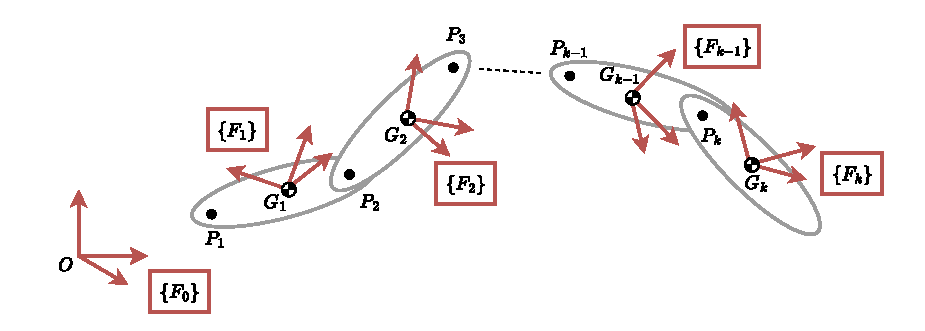
\includegraphics[trim={0 0 0 0},clip,width=1\linewidth]{img/chapter_4/general_rigid_body_model.pdf}
    \caption{Notations for a serial kinematic chain. The \emph{ground} $B_0$ is described via frame $\{F_0\}$ located at the origin $O$. A body $B_i$ is represented by a frame $\{F_i\}$ located at its center of mass $G_i$. Two bodies $B_{i-1}$ and $B_i$ are linked through a joint $J_i$ whose center is defined at point $P_i$. }
    \label{fig:general_rigid_body_model}
\end{figure}

A \emph{joint configuration} describes the specific positions of all the joints in a kinematic chain. It is defined by the values of the \emph{generalized coordinates}, which are parameters that quantify the different ways the joints can move.

Such serial kinematic chains assume that bodies are resistant to deformation, \emph{i.e.} they have infinite stiffness, and that joints' centers of rotation (points $P_1, \dots, P_k$) do not change their position for different joint configurations. However, this is not entirely sufficient for upper-limb modeling, as the scapulohumeral rythm affects internal forces, such as the glenohumeral joint force (\cite{flores-hernandezScapulothoracicRhythmAffects2019}). Since we focus on maximal forces produced at the hand of the upper limb, we need a more complex model to accurately capture essential biomechanical components required for further experimental validations. 

\subsubsection*{Actuators and muscle geometry}
While a serial kinematic chain can be actuated by controlling its joint torques or velocity, to better mimic human behavior, we should consider actuators. An actuator is a component that converts an energy source into motion. For instance, a cable-driven parallel robot could be powered by hydraulic cables. In the human body, muscles serve as actuators, converting chemical energy into mechanical force to produce movement.

The most commonly used muscle models are based on the Hill's model (\cite{hillHeatShorteningDynamic1938}). A Hill-type muscle model represents a musculotendon unit, comprising muscle fibers and a tendon, as a mechanical system with three interconnected elements. The contractile element simulates the active force generation of the muscle fibers.  A spring-like series elastic element, representing the tendon's elastic properties, is in series with the contractile element. Finally, a parallel elastic element accounts for the passive elasticity of the muscle tissue itself and acts in parallel with the other two elements. 

In order to study how a muscle acts on a joint to produce motion, muscle modeling requires consideration of two distinct aspects: the force amount and its line of action. These two facets are intrinsically linked through the force-length and force-velocity relationships, fundamental principles of biomechanics established in (\cite{hillHeatShorteningDynamic1938}). These relationships describe how muscle force varies depending on its length and velocity of contraction. Zajac summarizes these muscle properties in (\cite{zajacMuscleTendonProperties1989a}). However, while explicit computations can be formulated for the generated muscle force, determining the muscle line of action depends on factors such as muscle geometry, joint type, and surrounding anatomical structures. If the muscle geometry is determined to be similar to a single line segment (or straight cables), the action of the muscle onto a spherical joint of rotation center $P$ is quantifiable as a real vector $\tau\in \IR^3$ termed the \emph{muscle joint torque} and noted $\tau$. By considering $\mathbf{u}$ the normalized muscle line direction, $f$ the produced muscle force amount, and $A$ the orthogonal projection of $P$ onto the muscle line, then $\tau$ (in unit Newton-meter N$\cdot$m) is computed as 
\begin{align*}
    \tau = f\mathbf{u} \times (A - P)
\end{align*} 
where $\times$ is the cross product in $\IR^3$. To obtain the torque produced along a specific joint rotation axis $\omega\in \IR^3$, there suffices to compute $\omega \cdot \tau$, where $\cdot$ denotes the usual dot product. The distance $\| A - P \|$ is usually refered as the \emph{lever arm}, which represents the perpendicular distance from the joint center to the muscle's line of action.

While the line segment approximation for muscle geometry offers computational simplicity in calculating muscle joint torque, it fails to capture the complexities of more realistic muscle shapes.  To address this, a generalized coordinate approach can be employed. By defining the muscle length as a function of generalized coordinates, $l(\mathbf{q})$, the muscle joint torque, $\tau$, about a joint axis $\omega$ can be determined through the partial derivative of the length function with respect to the generalized coordinates:
\begin{align*}
    \tau = \frac{\partial l(\mathbf{q})}{\partial \mathbf{q}}
\end{align*}

This formulation accommodates any continuous muscle path, provided the length function is differentiable. However, differentiating this function can be challenging, often necessitating numerical differentiation techniques or optimization algorithms, as employed in OpenSim musculoskeletal modeling software (\cite{delpOpenSimOpenSourceSoftware2007}).

The choice between simplified and complex muscle geometries depends on the specific application and desired level of accuracy. For instance, (\cite{livetAutomaticSimplifiedApproach2022}) consider that muscles are described as successive rigid segments connected by \emph{via points}. In (\cite{kedadriaShoulderMusculoskeletalModel2023}), the authors highlights the benefits of refined muscle geometry modeling. Their study demonstrated that detailed representations of muscle fiber paths, particularly in the shoulder, yield muscle moment arms that more closely align with experimental cadaveric data from (\cite{acklandMomentArmsMuscles2008}) than those obtained through simplified segment approximations. This suggests that incorporating more realistic muscle geometries can enhance the accuracy and fidelity of musculoskeletal models. In this regard, we will therefore consider the general case of complex muscle geometry models.

Enhancing the efficiency of complex musculoskeletal computations, particularly those involving moment arm calculations, has driven the exploration of alternative approaches to muscle geometry modeling. However, recent research has investigated the use of polynomial functions to represent muscle length and moment arms.

For instance in (\cite{menegaldoMomentArmsMusculotendon2004}), the authors employed polynomials to model 43 lower limb muscles in the lower extremity musculoskeletal model developed in (\cite{delpInteractiveGraphicsbasedModel1990a}). Their analysis of the tibialis anterior muscle revealed a maximum error of 0.15 cm in the computed moment arm surface across a wide range of ankle and subtalar joint angles, with the largest errors occurring near the joint limits.  While this study focused on predicting muscle moments, it did not explicitly evaluated the accuracy of muscle length estimations.
In (\cite{sobinovApproximatingComplexMusculoskeletal2020}), the authors utilized higher-order polynomials (order 6) to represent upper limb muscles. Their findings indicated promising accuracy for both muscle length and moment arms across various joint configurations, with errors below 5$\%$ compared to geometric computations for both measures. However, despite their computational advantages, the authors noted that the accuracy of these polynomial models depended on the quality of the data used to generate them. Specifically, they observed increased force and torque errors with increasing noise levels in the input muscle length and moment arm data. For example, 10$\%$ noise in the input data resulted in a 7.36$\%$ error in produced force and a 61.2$\%$ error in torque compared to expected values.

To ensure the accurate representation of muscle action and align with experimental findings reported in the literature, this thesis will employ complex muscle geometries that reflect experimentally measured moment arm data. Furthermore, muscle force production will be modeled using the Hill-type model, a widely adopted and experimentally validated approach in the field of biomechanics.

\subsection{Force feasible sets formalism}
We now examine how muscles generate forces across joints to produce forces at the hand. This will lead to the characterization of the feasible force sets, which represent the range of forces that can be generated by the combined action of the upper limb muscles.

\subsubsection*{Tension feasible set}
In (\cite{hillHeatShorteningDynamic1938}), the author described initially a mechanical model of two components, one representing a muscle and the other a tendon. Combined into one system, these composants form the \emph{musculotendon unit}. Current Hill-based models comprise three components: 1) the \emph{contractile element} (CE), which corresponds to the contractile properties of fibers inside the muscle part; 2) the \emph{passive elastice element} (PEE), which encompasses the elastic properties of these fibers and is in parallel with the contractile element; and 3) the \emph{serial elastic element} (SEE), which reflects the elastic properties
of the tendon in the musculotendon unit and is series with the first two components. Figure \ref{fig:hill_mech_model} summarizes this model.
\begin{figure}[!htb]
    \captionsetup{justification=centering}
    \centering
    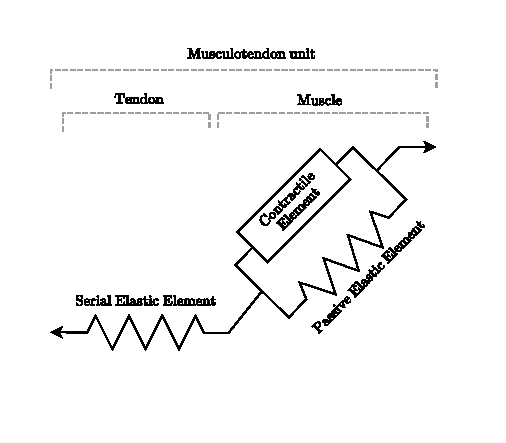
\includegraphics[trim={20 30 30 15}, clip, width=0.5\linewidth]{img/chapter_1/hill_mechanical_model.pdf}
    \caption{Hill's muscle model (\cite{hillHeatShorteningDynamic1938}). Forces exerted by a tendon are modeled via a spring is series with the muscle forces modeled in two parts: a contractile element in parallel with a spring.}
    \label{fig:hill_mech_model}
\end{figure}

Hill discovered a relationship between forces $f^M$ (in Newton) produced by a muscle and its length $l^M$ (also termed \emph{fiber} length) as well as its velocity $\dot(l^M)$. Since this thesis focuses on isometric condition, \emph{i.e.} $\dot{l^M} = 0$, we will describe the muscle force-length relationship only. For this, we consider the \emph{activation} of a muscle, \emph{i.e.} how much it should contract. The activation is controlled by a neural command, and is represented as a positive real value $a\in [0,1]$. In isometric condition, where activation is at $1$, the contractile element of a muscle produces its peak force $f_{iso}$, termed the \emph{maximal isometric force}, at a specific length $l_o$, the \emph{optimal fibel length}. When the contractile part has a smaller or larger length than $l_o$, the produced force decreases. For other activation states, this force is proportional to the activation. These relationships specifically describe the force produced by the contractile component of Hill's muscle model, which is termed the \emph{active force} $f_A$. The passive muscle element also exerts forces $f_P$, as it is modeled as a non-linear spring: these depends on the muscle length and are termed \emph{passive forces}. Since both active and passive forces are modeled in parallel, the total muscle force is the sum of their respective produced forces.
Figure \ref{fig:force_length_activation} describes these relations as curves.
\begin{figure}[!htb]
    \captionsetup{justification=centering}
    \begin{minipage}{0.49\linewidth}
        \centering
        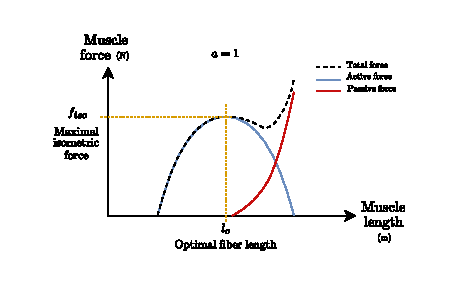
\includegraphics[trim={20 10 25 10}, clip, width=1\linewidth]{img/chapter_1/hill_force_length_relationship_fully_act.pdf}
    \end{minipage}
    \hfill
    \begin{minipage}{0.49\linewidth}
        \centering
        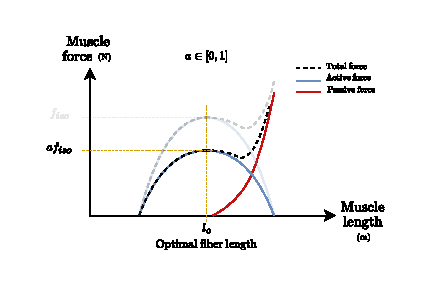
\includegraphics[trim={20 10 20 10}, clip, width=1\linewidth]{img/chapter_1/hill_force_length_relationship_all_act.pdf}
    \end{minipage}
    \caption{Simplification of Hill's force-length relationship in a muscle. When a muscle is fully activated ($a=1$, left figure), the muscle \emph{maximal isometric force} $f_{iso}$ is produced when the muscle length is at its \emph{optimal fiber length} $l_o$. In general (right figure), when the muscle activation varies, the active force-length curve is proportional to the activation, and so is the maximal force.}
    \label{fig:force_length_activation}
\end{figure}

However, the musculotendon unit is not a straight line, so to account for the non-linear shape of the musculotendon unit, both tendon and muscle are assumed to be separate segments with different lengths. The tendon is assumed to be bonded to the attaching bone, so that its produced force $f^T$ is along the bone's direction. In contrast, muscle fibers are \emph{pennated}, \emph{i.e.} there is a non-negligible angle $\alpha \in [0, \pi]$ between the tendon and the muscle segments. To account for this pennation angle, the produced muscle force $f^M$ is orthogonally projected onto the tendon's direction. 
\begin{figure}[!htb]
    \captionsetup{justification=centering}
    \centering
    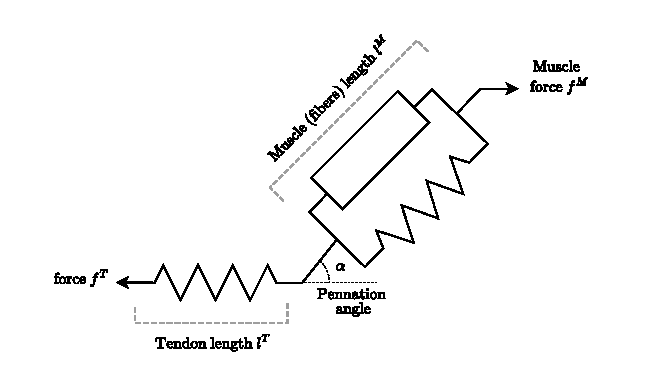
\includegraphics[trim={20 15 30 15}, clip, width=0.6\linewidth]{img/chapter_1/hill_mechanical_force_model.drawio.pdf}
    \caption{Forces in Hill's muscle model.}
    \label{fig:hill_mech_model_forces}
\end{figure}

When isometric conditions are assumed, the tendon force $f^T$ and muscle force $f^M$ are identical, and the muscle force-length relationship can be described as follows:
\begin{align*}
    f^M = f_{iso}(af_A(l^M) + f_P(l^M))\cos (\alpha)
\end{align*}
where $a\in [0,1]$ is the muscle activation, $\alpha\in [0, \pi]$ the pennation angle, $f_A$ is the normalized active force curve and $f_P$ is the normalized passive force curve, in which the given muscle lengths $l^M$ are normalized by the optimal fiber length $l_o$.

Another important muscle parameter is the tendon slack length $l_s$.
Tendons stretch and recoil during movement, and and because its force behavior is modeled as a spring, the tendon produces its own force $f^T$ depending on its own length $l^T$. Similarly to the passive elastic element of the muscle part, the tendon produces force when it is stretched beyond a certain length, termed the \emph{tendon slack length} and noted $l_s$.

However, in isometric conditions the forces occurring within the musculotendon unit balance each other, so that the muscle force equals the tendon force. Hill's model also incorporates muscle velocity and a force-velocity relationship, which describes how the force a muscle can generate depends on its speed of contraction. Elastic elements could also be considered to have visco-elastic properties, so that their velocities also influence their forces. However, this thesis focuses only on isometric conditions, so we do not need to consider any velocity-related properties for force-generation within the musculotendon unit.

It is to be noted that the forces generated within the musculotendon unit are considered positive when acting in their direction of application. The term \emph{tension} is therefore used to emphasize that these forces are always considered positive, acting in the direction that pulls on the tendon. 
% The biomechanical model of a muscle being defined in isometric conditions, we shall concentrate on explicitely descrbe the active and passive force-length curves.

% \paragraph*{The Hill-Thelen muscle model.}

The \emph{feasible tensions of a muscle} refer to the set of all tensions exertable by a muscle for a specific length. Since its tension depends on its length, the feasible tensions of a muscle reflect the possible tensions achievable solely through varying the activation level. When considering a musculoskeletal model and one of its muscle $M$, its feasible tension set is noted $\mathcal{T}^M$ and is defined as follows:
\begin{align*}
    \mathcal{T}^M &= \left\{ t\in \IR_{\geq 0} \mid t = f_{iso}(af_A(l^M) + f_P(l^M))\cos (\alpha),\quad a\in [0,1]\right\} \\
    &= [\underline{t^M}, \, \overline{t^M}]
\end{align*}
where $\underline{t}^M = \min \mathcal{T}^M$ and $\overline{t}^M = \max \mathcal{T}^M$. 

Since a musculoskeletal model may consist of multiple muscles, the \emph{tension feasible set} (of the musculoskeletal model) denotes all muscle tension combinations producible by all muscles. It is noted as $\mathcal{T}$ and is a subset of a $m$-dimensional real space, where $m$ is the number of considered muscles. This set depends on the specific posture of the musculoskeletal system, as muscle lengths change with joint angles.

Different combinations of muscle tensions reflect different biomechanical assumptions. For instance, if we define for a posture $\mathcal{T}$ as:
\begin{align*}
    \mathcal{T} = \left\{ \mathbf{t}=(t_1,\dots,t_m)\in\IR^m \mid t_i \in [\underline{t_i}, \, \overline{t_i}],\, \forall i=1,\dots, m \right\}
\end{align*} 
then $\mathcal{T}$ is a $m$-dimensional hyperrectangle, also termed $m$-\emph{orthotope} (\emph{c.f.} Figure \ref{fig:tension_set_orthotope_example}). This implies that all muscles can be fully activated at the same time.
\begin{figure}[!htb]
    \captionsetup{justification=centering}
    \centering
    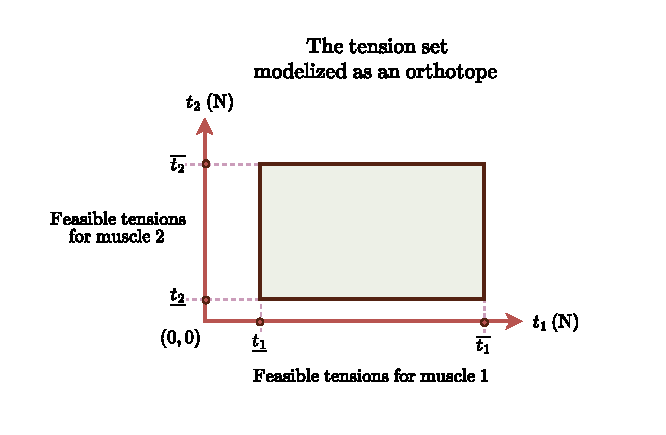
\includegraphics[trim={25 20 40 16}, clip, width=0.6\linewidth]{img/chapter_2/tension_set_orthotope.pdf}
    \caption{A muscle exerts a tension in a feasible range of values. The set of all tension combinations $\mathcal{T}$ is shaped as an \emph{orthotope} (or \emph{hyperrectangle}): it assumes muscles act independently from each other.}
    \label{fig:tension_set_orthotope_example}
\end{figure}

Having defined the tension feasible set, we will now formulate the force feasible set formulation by showing how the equation of motion relates muscle tensions to the forces produced at the hand.

\subsubsection*{The equation of motion}
In a dynamical context, the serial kinematic chain of a considered musculoskeletal model is described by $n$ generalized coordinates associated to $n$ degrees of freedom. We shall consider the parametrization of the degrees of freedom as a vector of \emph{generalized coordinates} $\mathbf{q} = (q_1, \dots, q_n)\in \IR^n$, and also consider the generalized velocities $\dot{\mathbf{q}} = (\dot{q}_1, \dots, \dot{q}_n)\in \IR^n$ and the generalized accelerations $\ddot{\mathbf{q}} = (\ddot{q}_1, \dots, \ddot{q}_n)\in \IR^n$. These vectors describe the kinematic chain's configuration and how it is changing over time. Each rigid body $B_i$, for $i = 1,\dots, k$ has a positive mass $m_i$ (in kg). To describe how this mass is distributed throughout the kinematic chain and how it affects the system's resistance to acceleration, we define the inertia matrix of the musculoskeletal model. Importantly, this matrix depends on the joint configuration $\mathbf{q}$. We denote by $C(\mathbf{q}, \dot{\mathbf{q}})$ the Coriolis and centrifugal torques. These are velocity-dependent forces that arise due to motions in the kinematic chain and the joints between its links. $\mathbf{G}(\mathbf{q}) \in \IR^n$ denotes the vector of gravitational torques.
Finally, $\tau\in \IR^n$ denotes the vector of \emph{joint torques} and describes the forces applied by the actuators at each joint to drive the motion.

The \emph{equation of motion} (\cite{lauGeneralizedModelingMultilink2013}; \cite{skuricCoupledViewPhysical}) is thus described as a differential equation of the generalized coordinates:
\begin{align*}
    M(\mathbf{q})\ddot{\mathbf{q}} + C(\dot{\mathbf{q}}, \mathbf{q})\dot{\mathbf{q}} + \mathbf{G}(\mathbf{q}) = \tau
\end{align*}

The surrounding space for $\tau$ vectors is termed the \emph{torque space}, and is of dimension the number of generalized coordinates, which we will assume is equal to the number of degrees of freedom.
Joint torque vectors $\tau$ are produced by actuators and other forces in the musculoskeletal model. 

On one hand, a force $\mathbf{f}$ applied at an end-effector point $X = (x_1, x_2, x_3)\in \IR^3$ is projected linearly onto the torque space. Indeed, the Jacobian matrix at point $X$ for joint configuration $\mathbf{q}$, $J_X(\mathbf{q})\in \IR^{3\times n}$, which relates the velocities of the generalized coordinates $\dot{\mathbf{q}}$ to the Cartesian velocities of the end-effector $\dot{X}$, describes how a change in the generalized coordinates results in a change of a Cartesian position:
\begin{align*}
    \dot{X} = J_X(\mathbf{q})\dot{\mathbf{q}}
\end{align*}
where $J_X(\mathbf{q}) = \left(\frac{\partial x_i}{\partial q_j}\right)_{i,j}$ for $i=1,2,3$ and $j=1,\dots, n$. Due to kineto-static duality, which relates forces and velocities in a mechanical system, the transpose of $J_X(\mathbf{q})$, noted $J_X^T(\mathbf{q})$ relates a linear force $\mathbf{f}\in\IR^3$ at $X$ to the joint torques as follows:
\begin{align*}
    \tau = J_X^T(\mathbf{q})\mathbf{f}
\end{align*}

On the other hand, the length $l_i$ of muscle $i$, for $i=1,\dots, m$, depends on the joint configuration $\mathbf{q}$. The muscle velocities $\dot{\mathbf{l}} = (\dot{l}_1, \dots, \dot{l}_m)\in \IR^m$ are described through the linear mapping $L\in\IR^{m\times n}$, which relates the rates of change of muscle lengths to the velocities of the generalized coordinates: 
\begin{align*}
    \dot{\mathbf{l}} = L(\mathbf{q})\dot{\mathbf{q}}
\end{align*}
where $L(\mathbf{q}) = \left(\frac{\partial l_i}{\partial q_j}\right)_{i,j}$ for $i=1,\dots, m$ and $j=1,\dots, n$. $L$ is termed the \emph{lever arm} matrix. Similarly to the Jacobian matrix, the transpose of $L$ relates the muscle tensions $\mathbf{t}\in\IR^m$ to the joint torques via:
\begin{align*}
    \tau = -L^T(\mathbf{q})\mathbf{t}
\end{align*}
The negative sign in this equation reflects the sign convention used for muscle forces and joint torques. For instance, when the biceps muscle contracts (positive tension), it creates a flexion torque at the elbow, which is represented as a negative torque in the equation since the positive direction for the elbow angle is extension

When no other actuators or forces are considered, the equation of motion is written as:
\begin{align*}
% \label{eq:equa_motions_muscle}
    M(\mathbf{q})\ddot{\mathbf{q}} + C(\dot{\mathbf{q}}, \mathbf{q})\dot{\mathbf{q}} + \mathbf{G}(\mathbf{q}) + J_X^T(\mathbf{q})\mathbf{f} = -L^T(\mathbf{q})\mathbf{t}
\end{align*}

We will now formulate the force feasible set, for both dynamic and static cases.

\subsubsection*{General formulation of force feasible sets}
As described in (\cite{skuricCoupledViewPhysical}), the \emph{force feasible set} $\mathcal{F}_X^{\mathcal{T}}(\mathbf{q}, \dot{\mathbf{q}}, \ddot{\mathbf{q}})$ at joint configuration $(\mathbf{q}, \dot{\mathbf{q}}, \ddot{\mathbf{q}})$ is defined to be the set of all forces $\mathbf{f}(\mathbf{q}, \dot{\mathbf{q}}, \ddot{\mathbf{q}})$ such that there exist muscle tensions satisfying the equation of motion:
\begin{align*}
% \label{eq:ffs_general}
    \mathcal{F}_X^{\mathcal{T}}(\mathbf{q}, \dot{\mathbf{q}}, \ddot{\mathbf{q}}) = \left\{\mathbf{f}\in\IR^3 \mid \exists \mathbf{t}\in \mathcal{T}(\mathbf{q}, \dot{\mathbf{q}}),\, M(\mathbf{q})\ddot{\mathbf{q}} + C(\dot{\mathbf{q}}, \mathbf{q})\dot{\mathbf{q}} + \mathbf{G}(\mathbf{q}) + J_X^T(\mathbf{q})\mathbf{f} = -L^T(\mathbf{q})\mathbf{t}\right\}
\end{align*}

\subsubsection*{Force feasible sets in isometric conditions}
In \emph{isometric conditions}, muscles are contracting but are not shortening or lengthening, meaning the musculotendon forces are in a static equilibrium state where the generalized velocities and accelerations of the kinematic chain are $\dot{\mathbf{q}}=0$ and $\ddot{\mathbf{q}} = 0$. We use the term \emph{posture} to refer to a joint configuration $\mathbf{q}$ where the velocities and accelerations are null.

Force feasible sets in isometric conditions are described for a given posture $\mathbf{q}$ as follows:
\begin{align*}
% \label{eq:ffs_description_static}
    \mathcal{F}_X^{\mathcal{T}}(\mathbf{q}) = \left\{\mathbf{f}\in\IR^3 \mid \exists \mathbf{t}\in \mathcal{T}(\mathbf{q}), \quad \mathbf{G}(\mathbf{q}) + J_X^T(\mathbf{q})\mathbf{f} = -L^T(\mathbf{q})\mathbf{t} \right\}
\end{align*}

It corresponds to the set of forces applied at the end effector such that the gravity and a combination of muscle forces can compensate for the applied force. Throughout this thesis, the term \emph{force feasible set} will be used exclusively to refer to the \emph{force feasible set in isometric conditions}. 

Before delving into force feasible set computations, we introduce more compact notations to improve readability. When possible, we will denote a force feasible set $\mathcal{F}_X^{\mathcal{T}}(\mathbf{q})$ as $\mathcal{F}(\mathbf{q})$, and simply as $\mathcal{F}$ when the posture is clear from the context or not relevant. Since the relevant tension feasible set will always be defined beforehand, the subscript $\mathcal{T}$ can be omitted. Furthermore, forces will generally be applied at the right hand of an upper-limb musculoskeletal model, since this thesis focuses exclusively on forces applied at the right hand. The coordinates of $X$ will be specified when relevant, such as during \emph{in silico} or \emph{in vivo} experiments. However, even when the coordinates of $X$ are specified, the $X$ subscript will be omitted from the force feasible set notation. Thereforce, $\mathcal{F}(\mathbf{q})$ will always denote a force feasible set with an underlying tension feasible set (defined beforehand) and a point of application $X$. Consequently, it is also common to denote the Jacobian transpose computed at point $X$ as $J^T(\mathbf{q})$, omitting the $X$ subscript.

Since the force feasible set depends on the posture $\mathbf{q}$, it is often expressed as a function of $\mathbf{q}$. This highlights the fact that the set of feasible forces changes as the posture changes. For brevity, we will often omit the explicit dependence on $\mathbf{q}$ in the notation for force feasible sets, where it is understood that all elements in the set's definition implicitly depend on $\mathbf{q}$:
\begin{align*}
    \mathcal{F} = \left\{\mathbf{f}\in\IR^3 \mid \exists \mathbf{t}\in \mathcal{T}, \quad J^T\mathbf{f} = -L^T\mathbf{t} - \mathbf{G}\right\}
\end{align*}

The force feasible set formulation is a geometric transformation of the tension feasible set $\mathcal{T}$. To highlight the underlying geometry, we can express this relationship in an alternative form. Let $\mathcal{F}$ be the force feasible set at end-effector $X$ for a given posture and a tension feasible set $\mathcal{T}$. Then, $\mathcal{F}$ can be expressed, up to linear transformation, as:
\begin{align*}
    \im{J^T} \cap \left(-L^T\mathcal{T}-\mathbf{G}\right)
\end{align*}
where $-L^T\mathcal{T}-\mathbf{G} = \left\{\tau\in \IR^n\mid \exists \mathbf{t}\in\mathcal{T},\quad \tau = -L^T\mathbf{t} - \mathbf{G} \right\}$ is the \emph{torque feasible set} and representing all torques achievable through muscle tensions and gravity. Also, $\im{J^T}$ denotes the \emph{image} of the matrix $J^T$, which is the vector space spanned by its columns. We will assume that $\dim \im{J^T}$ is $3$, or more generally, $p$, where $p$ is the rank of $J^T$. Therefore, $\im{J^T}$ is a subspace of the $n$-dimensional torque space. If $J^T$ is invertible, then $\im{J^T}$ spans the entire torque space. This implies that every exertable force at the end-effector corresponds to a unique combination of joint torques, indicating no redundancy in the system.

The sets $\mathcal{F}$ and $\im{J^T} \cap \left(-L^T\mathcal{T}-\mathbf{G}\right)$ are considered \emph{equivalent up to linear transformation}. This means that they are not \emph{strictly} identical, but they represent the same underlying set viewed from two different perspectives: the Cartesian force space, where forces are expressed in Cartesian coordinates ($\mathbf{f}\in \IR^3$), and the torque space, where they are expressed as joint torques ($J^T\mathbf{f}\in \IR^n$). When expressed in the torque space, the force feasible set $\mathcal{F}$ becomes $J^T\mathcal{F} := \left\{\tau\in \IR^n \mid \exists \mathbf{f}\in \mathcal{F}, \quad \tau = J^T\mathbf{f}\right\}$. 
To map forces from the torque space back to the Cartesian force space, we can use the \emph{Moore-Penrose pseudo-inverse of $J^T$}, denoted $(J^T)^+$, and we have $\mathcal{F} = (J^T)^+(J^T\mathcal{F})$, which recovers the original force feasible set in Cartesian coordinates. The (left) Moore-Penrose pseudo-inverse $(J^T)^+$ is defined as:
\begin{align*}
    (J^T)^+ = (JJ^T)^{-1}J
\end{align*}
which satisfies the property $(J^T)^+J^T = I_3$, where $I_3$ is the $3\times 3$ identity matrix.

For conciseness, we can consider the force feasible set $\mathcal{F}$ in either the Cartesian force space or the torque space. This is justified by the fact that an invertible linear transformation, which can be computed for any given posture, allows us to seamlessly switch between these two representations.

\subsection{Force feasible sets computation}
Given a tension feasible set $\mathcal{T}$, the force feasible set $\mathcal{F}$ can be described as two successive geometric operations: a \emph{projection} of $\mathcal{T}$ onto the torque space, creating the \emph{torque feasible set}, which is then \emph{intersected} by $\im{J^T}$, yielding the force feasible set $\mathcal{F}$ expressed in the torque space (\cite{skuricCoupledViewPhysical}). This modeling of forces is based on a rigid-body framework, which may not fully capture the complexities of deformable systems. Nevertheless, we assume throughout this thesis that bones are non-deformable. The force feasible set geometric construction can be summarized as follows:
\begin{figure}[!ht]
    \centering
    \captionsetup{justification=centering}
    \begin{tikzcd}
        \mathcal{T} \arrow[rr, "\text{projection}"'] &  & -L^T\mathcal{T}-\mathbf{G} \arrow[rr, "\text{intersection}"'] &  & J^T\mathcal{F} \arrow[r, "(J^T)^+"', bend right] & \mathcal{F} \arrow[l, "J^T"', bend right]
    \end{tikzcd}
    % \caption{Description of the geometric operations to derive the force feasible set in isometric conditions. The set of muscle tensions $\mathcal{T}$ is projected and translated onto the torque space to create the torque feasible set $\mathcal{T}_o$. It is then intersected with a vector space ($\im J^T$) to produce the force feasible set $\mathcal{F}$ described in the torque space, or conveniently in the Cartesian force space using $(J^T)^+$. In practice, we prefer to express $\mathcal{F}$ in the torque space since $(J^T)^+$ is a bijection between $\mathcal{F}$ and $\mathcal{F}'$.}
    % \label{fig:segsd}
\end{figure}

Throughout this thesis, we use the term \emph{projection} in a generalized sense to highlight that the muscle tension space is related to the torque space through a surjective affine mapping, which consists of a surjective linear mapping ($-L^T$) followed by a translation ($-\mathbf{G}$). 
Since this mapping is surjective, the dimension of the torque space is less than that of the muscle tension space, implying that there are more muscles than degrees of freedom. The use of the term \emph{projection} here emphasizes the surjective nature of this mapping and should not be confused with the typical notion of an orthogonal projection.

The \emph{projection-intersection} process described above involves two main computations: projecting the tension feasible set onto the torque space and intersecting the resulting set with the image of the Jacobian transpose. Each of these computations requires distinct techniques, largely determined by the geometry of the tension feasible set $\mathcal{T}$.

If we assume that $\mathcal{T}$ is a cube or an orthotope, then $\mathcal{F}$ is a \emph{bounded convex polytope} (or simply \emph{polytope}), which is a generalization of a 2D convex polygon to $n$ dimensions (\cite{grunbaumConvexPolytopes2013}). A set is \emph{convex} if the line segment connecting any two points in the set is also contained within the set. A set is \emph{bounded} if it can be contained in a ball of finite radius. A polytope, by definition, includes all of its interior points as well as the points on its surface. 

Alternatively, the tension feasible set $\mathcal{T}$ could be a ball or an ellipsoid, which includes all of its interior points. In this case, the boundary of the force feasible set is an ellipsoid. Figure \ref{fig:tension_models_on_ffs} summarizes these different constructions.

\begin{minipage}{0.4\linewidth}
    \centering
    $\mathcal{T}$ is a cube, so $\mathcal{F}$ is a polytope.
\end{minipage}
\hfill
\begin{minipage}{0.4\linewidth}
    \centering
    $\mathcal{T}$ is a ball, so $\mathcal{F}$ is an ellipsoid.
\end{minipage}
\begin{figure}[!htb]
    \centering
    \captionsetup{justification=centering}
    \begin{minipage}{0.48\linewidth}
        \centering
        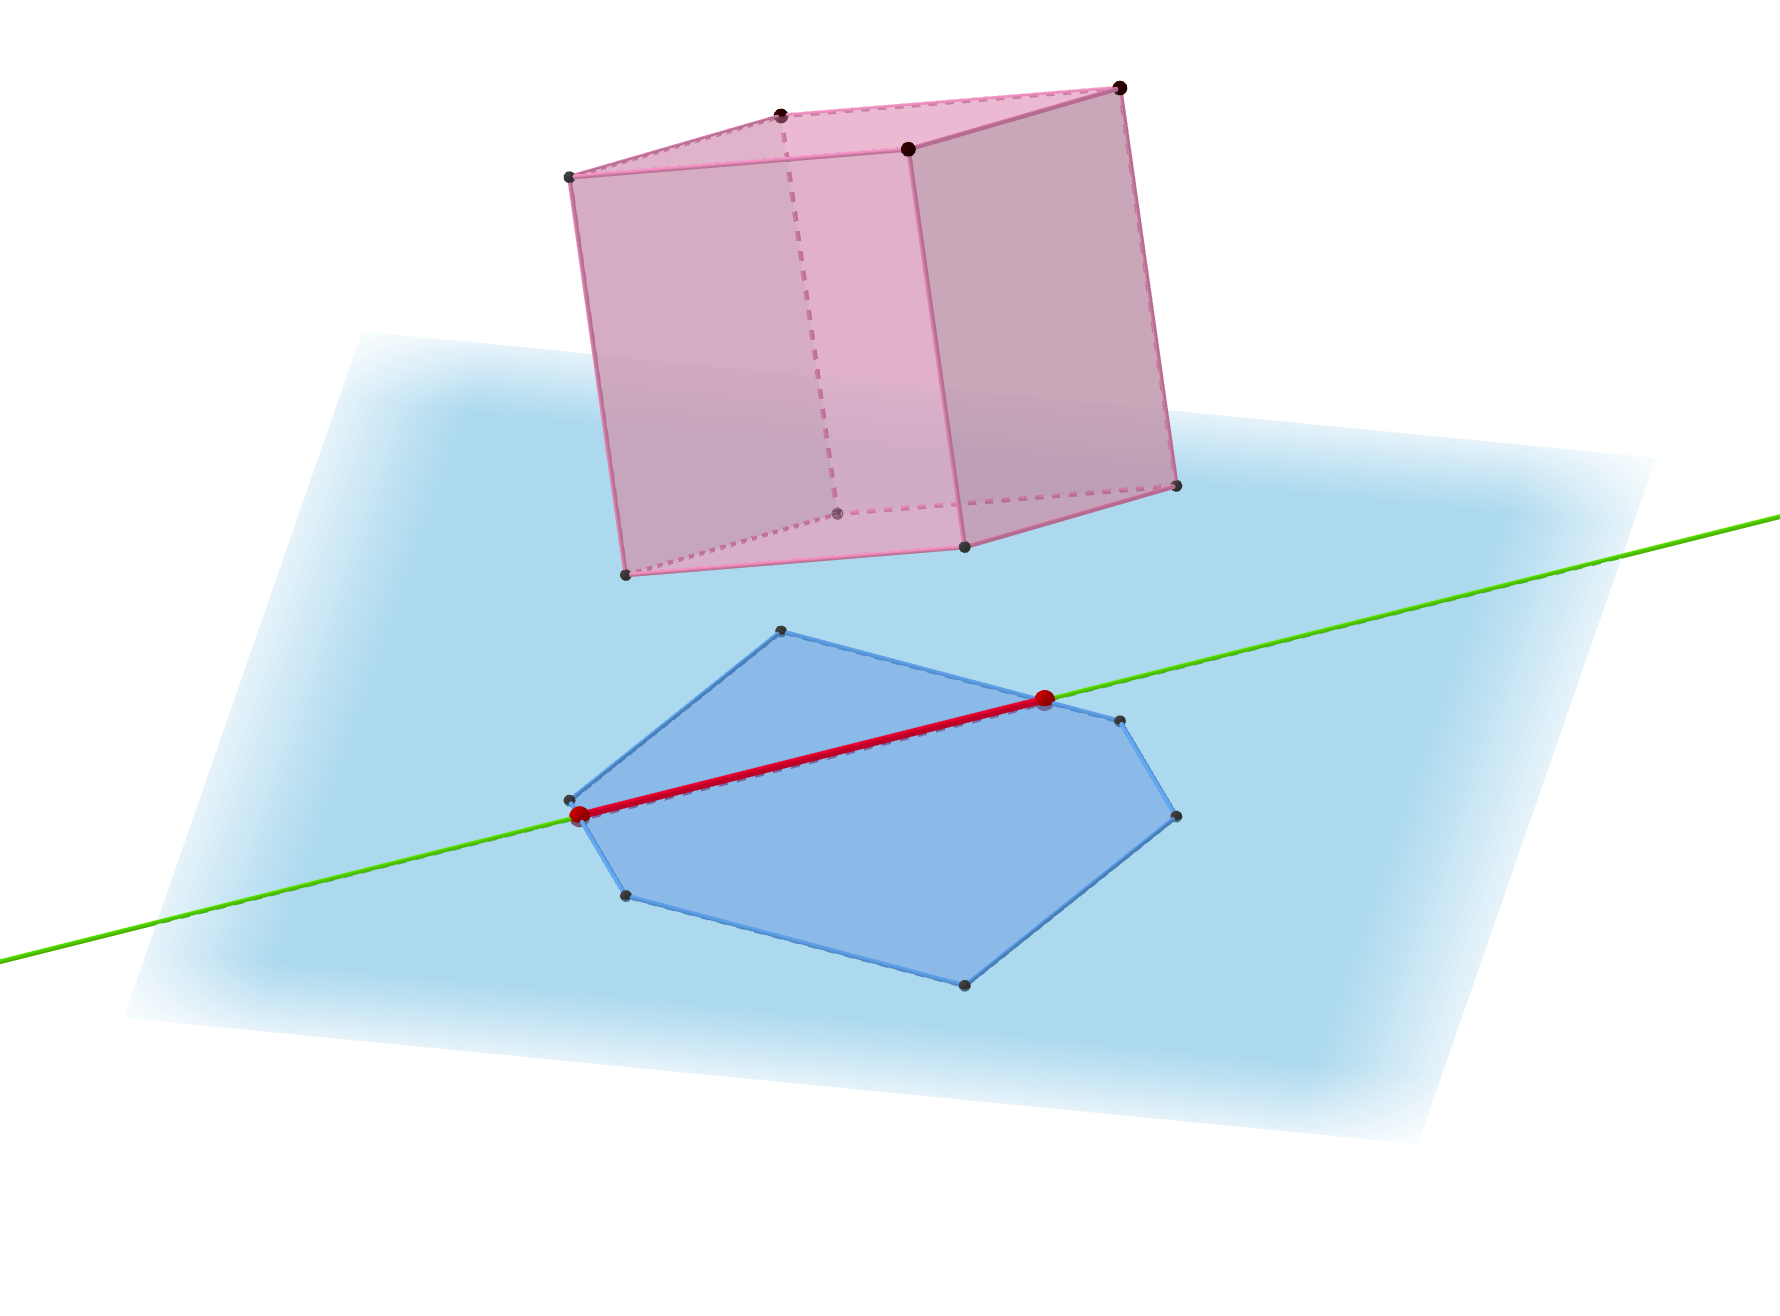
\includegraphics[trim={50 150 50 70}, clip, width=1\linewidth]{img/chapter_3/polytope_better_ggb.png}
    \end{minipage}
    \hfill
    \begin{minipage}{0.48\linewidth}
        \captionsetup{justification=centering}
        \centering
        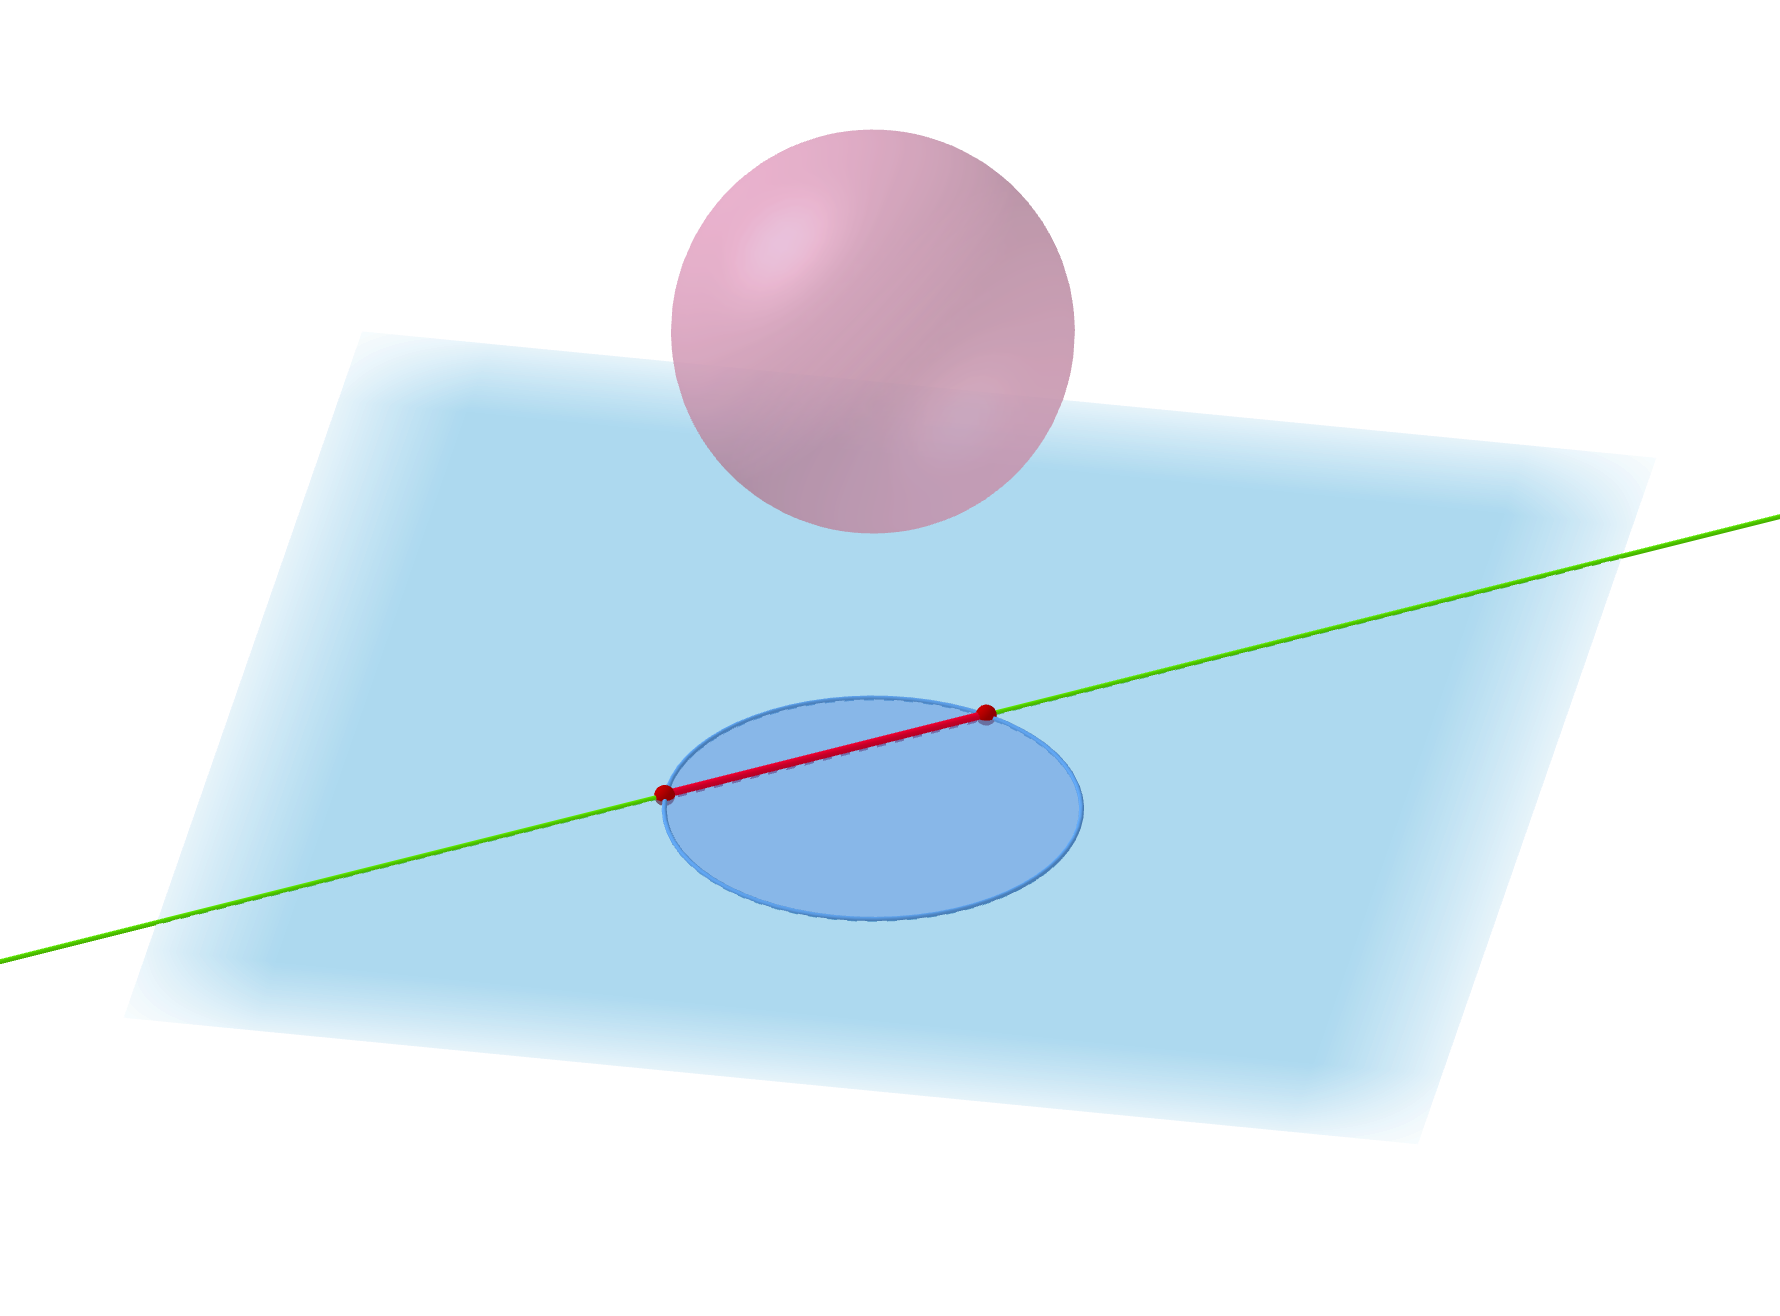
\includegraphics[trim={50 150 50 70}, clip, width=1\linewidth]{img/chapter_3/polytope_from_sphere_ggb.png}
    \end{minipage}
    \caption{Force feasible set $\mathcal{F}$ (red) resulting from different tension feasible sets $\mathcal{T}$ (pink). The blue shape represents the torque feasible set, and the green line represents $\im{J^T}$.}
    \label{fig:tension_models_on_ffs}
\end{figure}

We will now detail how to explicitly compute force feasible sets for both polytopic and ellipsoidal constructions.

\subsubsection*{Representing force polytopes}
When the tension feasible set $\mathcal{T}$ is an orthotope (a generalization of a rectangle to higher dimensions), the force feasible set $\mathcal{F}$ is a \emph{force polytope}. Polytopes have two main distinct representations: the $\mathcal{V}$-representation, which describes the polytope by its vertices, and the $\mathcal{H}$-representation, which describes it by its supporting hyperplanes.

The $\mathcal{V}$-representation of a polytope consists of its extremal points, commonly known as \emph{vertices}. Any point that can be expressed as a weighted average of these vertices is necessarily included in the polytope, as stated by Caratheodory's theorem (\cite{caratheodoryUberVariabilitatsbereichFourierschen1911}). The set of all possible weighted averages of two or more vertices is called the \emph{convex hull} of those vertices. In contrast, the $\mathcal{H}$-representation describes a polytope as the intersection of multiple half-spaces. Each half-space is defined by a linear inequality. Therefore, the $\mathcal{H}$-representation essentially consists of a set of linear inequalities that define the polytope's faces and determine which side of each face belongs to the polytope. Specifically, each face of a polytope can be represented by a \emph{hyperplane} (\cite{grunbaumConvexPolytopes2013}), which is an $(n-1$)-dimensional subspace of an $n$-dimensional space. Figure \ref{fig:polytope_v_and_h_rep} presents simple 2D examples of both representations.
\begin{figure}[!htb]
    \captionsetup{justification=centering}
    \begin{minipage}{0.49\linewidth}
        \centering
        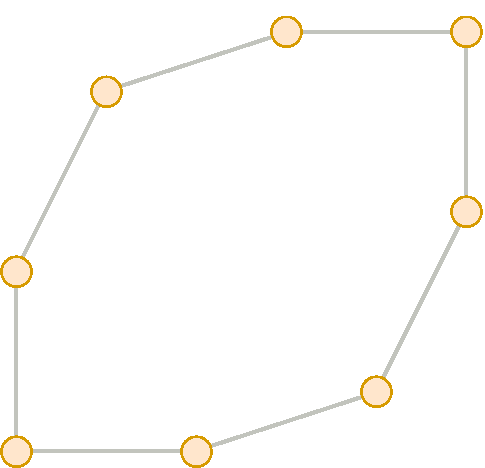
\includegraphics[trim={0 0 0 0},clip, width=0.6\linewidth]{img/chapter_2/zonotope_vertices.pdf}
    \end{minipage}
    \hfill
    \begin{minipage}{0.49\linewidth}
        \centering
        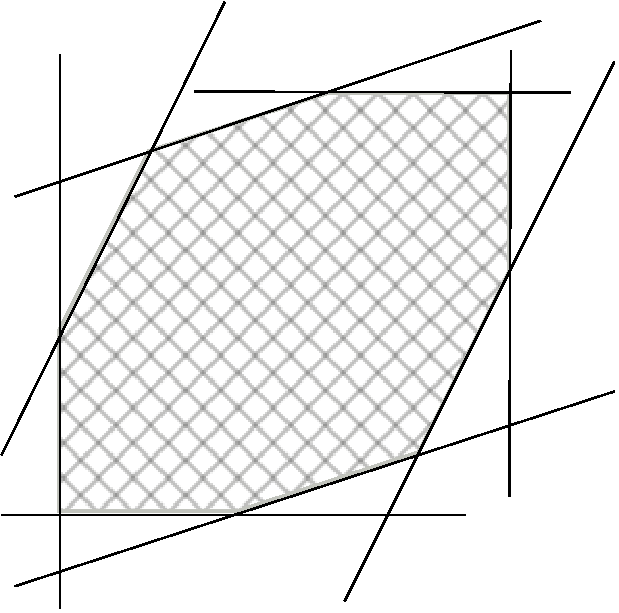
\includegraphics[trim={0 0 0 0},clip,width=0.75\linewidth]{img/chapter_2/zonotope_hyperplanes.pdf}
    \end{minipage}
    \caption{Polytope representations: A polytope can be described according to its vertices (the $\mathcal{V}$-representation) or by halfspaces determined from its bounding hyperplanes (the $\mathcal{H}$-representation).}
    \label{fig:polytope_v_and_h_rep}
\end{figure}

The $\mathcal{V}$- and $\mathcal{H}$-representations are equivalent when a polytope is \emph{full-dimensional} (\cite{grunbaumConvexPolytopes2013}), meaning it has the same dimension as the \emph{ambient} space. An ambient space refers to the surrounding space in which the polytope is described. When a polytope is full-dimensional, this is equivalent to saying that the polytope is not \emph{flat} in the ambient space. For instance, a polygon in a 3D space is not full-dimensional and is considered \emph{degenerate}. Force polytopes, when expressed in the torque space, are often degenerate, specifically when the rank of $\im{J^T}$ is strictly less than the dimension of the torque space, as shown in figure \ref{fig:ffs_when_tension_set_orthotope}.
\begin{figure}[!htb]
    \captionsetup{justification=centering}
    \centering
    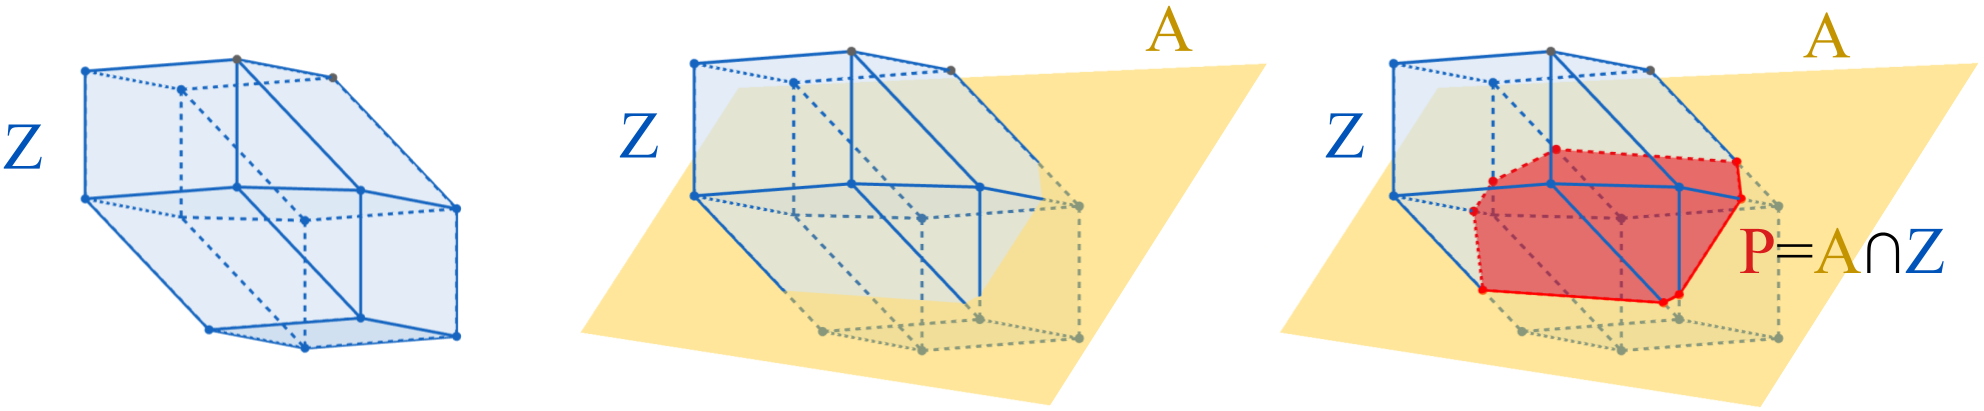
\includegraphics[trim={0 0 0 0}, clip, width=1\linewidth]{img/chapter_1/Polytope inter.png}
    \caption{Construction of a force polytope $P$ from a tension orthotope $\mathcal{T}$. $\mathcal{T}$ is projected onto the 3D torque space ($Z$), then intersected with the 2D subspace $\im{J^T}$ ($A$). The resulting force polytope P is degenerate as it is 2-dimensional within the 3D ambient torque space.}
    \label{fig:ffs_when_tension_set_orthotope}
\end{figure}

The $\mathcal{V}$- and $\mathcal{H}$-representations are the most common, as they encapsulate crucial information that force polytope construction does not share at first sight: they characterize a polytope's \emph{surface}. So, in order to visualize a 3D force polytope, a correspondence from the projection-intersection description should be made to either its vertices or bounding hyperplanes. Either representation would suffice, as algorithms already exist to convert from the $\mathcal{V}$- to the $\mathcal{H}$-representation, as described in (\cite{avisPivotingAlgorithmConvex}).

One approach is to explicitly compute the $\mathcal{H}$-representation of the torque feasible set, which is the projection of the tension feasible orthotope onto the torque space. Numerous algorithms exist for this purpose, such as the \emph{Hyperplane-Shifting method} (\cite{gouttefardeCharacterizationParallelManipulator2010a}) for describing the bounding hyperplanes, or the algorithms proposed in (\cite{radaNewAlgorithmEnumeration2018}) and (\cite{guCounterfactualIdentificationLatent2022}) for enumerating the vertices. Next, we need to compute the polytope that results from intersecting this torque feasible set with $\im{J^T}$. Once we have the bounding hyperplanes of the torque feasible set, we intersect each of them with $\im{J^T}$. This creates a new set of half-spaces within $\im{J^T}$. The force polytope is then defined as the smallest polytope enclosed by these new half-spaces. The Fourier-Motzkin elimination method can be used to obtain this new set of half-spaces, as it is specifically designed to find the smallest polytope enclosed by a given set of hyperplanes (\cite{dahlCombinatorialPropertiesFourierMotzkin2007}).

Although this direct approach is theoretically feasible, it is often impractical due to the high computational cost. Most algorithms for computing the $\mathcal{V}$-representation or $\mathcal{H}$-representation of polytopes are combinatorially complex, meaning their time complexity increases exponentially with the dimension of the muscle tension space. In Chapter \ref{chapter:2}, we will further demonstrate this computational challenge by benchmarking various algorithms for projecting the tension orthotope onto the torque space. We will also propose a new edge-based algorithm for efficiently describing the surface of the torque feasible set, leveraging its representation as a projection of an orthotope. Even with efficient algorithms, any exact description of the torque feasible set's surface will inevitably suffer from combinatorial complexity. Therefore, to avoid this computational bottleneck, approximation algorithms are often preferred for computing points on the polytope's surface. One such example is the \emph{Iterative Convex Hull} method proposed in (\cite{skuricOnLineFeasibleWrench2022}).

Beyond the $\mathcal{V}$- and $\mathcal{H}$-representations, there are many other possible polytope representations that capture specific polytope properties, just as the $\mathcal{V}$- and $\mathcal{H}$-representations encapsulate surface properties. For example, the \emph{Ehrhart quasi-polynomial} of a polytope $P$ is a polynomial of a positive variable $t$ that counts the number of integer points within a dilation $tP$ of the polytope. However, computing the coefficients of these polynomials is computationally expensive, with the combinatorial complexity increasing significantly as the number of vertices and the dimension of the polytope increase (\cite{barvinokComputingEhrhartQuasipolynomial2005}). A more practical representation is the \emph{constrained zonotope} representation, introduced in (\cite{scottConstrainedZonotopesNew2016}). The authors showed that any polytope can be constructed by intersecting a hypercube with a linear subspace and then projecting the result onto another subspace. Although this result was previously proven in (\cite{naumannBeliebigeKonvexePolytope1956}) and discussed by Grünbaum in (\cite{grunbaumConvexPolytopes2013}), it remains largely theoretical, with no explicit construction method provided. In Chapter \ref{chapter:3}, we leverage this result by demonstrating how to transform the projection-intersection description of a polytope (as we have enunciated for force polytopes) into an intersection-projection description. We provide an explicit method for this transformation. Our result is quite general, as it applies to any convex set constructed in this way, including arbitrary force feasible sets derived from convex tension feasible sets. The primary goal of this geometric inversion is to re-express linear constraints in the torque space as linear constraints in the muscle tension space. This is useful for geometrically identifying the muscles that are primarily responsible for generating forces at the end-effector.

\subsubsection*{Representing force ellipsoids}
A \emph{force ellipsoid} is a force feasible set that results from assuming the tension feasible set is an ellipsoid. This provides an alternative representation of force feasible sets, as demonstrated in (\cite{chiacchioForcePolytopeForce1997}), who used it to characterize the manipulability of a serial robot. In the context of biomechanics, this representation implies that the tension a muscle can exert depends on the tensions of all other muscles in the system. Specifically, the vector of muscle tensions must lie within an ellipsoid in the muscle tension space.

Whereas characterizing the surface of force polytopes is computationally challenging, force ellipsoids are much easier to compute and do not involve combinatorial complexity. This simplicity stems from the fact that both projections and intersections of ellipsoids with vector spaces result in ellipsoids (\cite{grunbaumConvexPolytopes2013}).

Any ellipsoid can be represented as an affine transformation of a unit sphere. Let $\mathcal{E}$ be an ellipsoid in $\IR^m$ and let $\mathcal{S}$ denote the unit sphere in $\IR^m$. Then, there exists a matrix $T\in\IR^{m\times m}$ and a vector $\mathbf{t}\in\IR^m$ such that:
\begin{align*}
    \mathcal{E} = T\mathcal{S} + \mathbf{t} = \left\{ \mathbf{x}\in\IR^m \mid \mathbf{x} = T\mathbf{u} + \mathbf{t}, \quad \|\mathbf{u}\|_2 = 1 \right\}
\end{align*}
where $\| \cdot \|_2$ denotes the usual Euclidean norm in $\IR^m$. 

Any linear transformation $T$ can be decomposed into three parts: 1) a rotation; 2) an \emph{anisotropic dilation}, which scales the sphere by different factors along its principal axes; 3) another rotation. This is known as the \emph{singular value decomposition} (SVD) of a linear transformation. The SVD provides a geometric interpretation of how the linear transformation $T$ deforms a unit sphere. Recall that the torque feasible set is obtained by projecting the tension ellipsoid onto the torque space. Since the projection is a linear transformation, and the composition of linear transformations is another linear transformation, the resulting torque feasible set is also an ellipsoid. However, the intersection of an ellipsoid with a vector space requires a more involved computation. In (\cite{sasakiHigherDimensionalSpatial2010a}), the authors offer a mathematical method to compute such an intersection.

Both the projection and intersection operations involve only matrix operations and vector translations. Therefore, force ellipsoids offer a significant computational advantage over force polytopes, which require addressing combinatorial problems.

\subsection{Conclusion}
In this section, we first described how a human upper limb can be represented \emph{in silico} using a model of a serial kinematic chain and muscles. This model allowed us to analyze the dynamics of the upper limb, which are captured by the \emph{equation of motion}. This equation relates the generalized coordinates, their velocities, and accelerations within the torque space. We considered both internal and external forces acting on the system. The internal forces are the muscle forces, and the external forces are those applied at the end-effector (the hand). We then expressed these forces in the torque space to incorporate them into the equation of motion. This led to the mathematical definition of the \emph{force feasible set} as the set of all external forces that can be applied at the end-effector while satisfying the equation of motion.

To analyze the force capabilities of the upper limb in static postures, we focused on force feasible sets in \emph{isometric} conditions, where the generalized velocities and accelerations are zero, and the musculotendon units are in equilibrium, meaning there is no movement. This allows for a more succinct representation of the force feasible sets, as the terms related to mass inertia and Coriolis accelerations in the equation of motion can be eliminated. We also presented a geometric interpretation of force feasible sets, highlighting their construction through a linear projection followed by an intersection with a vector space. These two operations are fundamental in set theory and have been extensively studied in the literature (\cite{bourbakiTheorieEnsembles2006}; \cite{dorstGeometricAlgebraComputer2007}).

However, even when assuming that the geometric construction of the force feasible sets depends only on convex sets - which is advantageous since a convex set is fully determined by its surface - we observed that the process of projecting and then intersecting introduces significant complexity in characterizing the surface of the resulting set. As examples, two common force feasible set representations were compared in terms of computing difficulties: force polytopes and force ellipsoids. Both characterization as polytopes and ellipsoids have been extensively studied in the literature (\cite{grunbaumConvexPolytopes2013}; \cite{artstein-avidanAsymptoticGeometricAnalysis2015}), and the projection-intersection problem is well-understood for both cases. However, the ellipsoid representation offers a significant computational advantage, as it involves only linear algebra operations.

It is important to consider other geometric characterizations of force feasible sets because, as we will see in Section \ref{sec:modeling_muscle_tensions}, the polytope and ellipsoid approaches have limitations in capturing the complex interactions between muscle tensions. Modeling the interactions between muscle tensions leads to a specific shape for the tension feasible set, which in turn influences the shape of the force feasible set. Chapter \ref{chapter:3} is dedicated to this problem, specifically addressing the case of a complex upper-limb muscular structure with a high number of muscles. In Chapter \ref{chapter:3}, we will show that for a complex musculoskeletal model, force polytope and ellipsoid representations are likely to be equivalent up to dilation. This means that the shape of any force feasible set is essentially the same ellipsoid but with a different scale, provided the muscle tension feasible set is convex and of sufficiently high dimension. While this theoretical result assumes a sufficiently large dimension for the muscle tension space, one of the objectives in Chapter \ref{chapter:4} will be to quantify how ellipsoid representations can be equivalent to polytopes in a muscle personalization process, even when only 50 muscles are considered, as the upper-limb musculoskeletal model in (\cite{holzbaurModelUpperExtremity2005}).

In the next section, we will explore the limitations of different force feasible set representations in a biomechanical context, comparing them to measured maximal isometric forces.

\section{Modeling force feasible sets via maximal isometric force measurements}
\label{sec:modeling_muscle_tensions}

As demonstrated by force polytopes and ellipsoids, the shape of a force feasible set is influenced by the shape of the tension feasible set. This section examines the underlying geometric assumptions about tension and torque feasible sets found in the literature and explores how these assumptions translate into biomechanical considerations for the muscles.

This section highlights how the limited diversity of tension interaction models hinders the accurate modeling of force feasible sets in the human upper limb. This limitation arises from the computational challenges involved in considering different tension feasible set shapes. Cable-driven parallel robots, which form the basis of musculoskeletal models, are not necessarily limited by modeling constraints, as their force feasible sets can be arbitrarily defined. However, in a human upper-limb, experimental measurements of maximal isometric force exertions reveal inconsistencies with current force feasible set representations. Specifically, force ellipsoids tend to underestimate the measured forces, while force polytopes tend to overestimate them (\cite{rezzougUpperLimbIsometricForce2021b}).

To examine these disagreements, subsection \ref{subsec:ffs_in_human_upper_limb} details the experimental process required for measuring maximal isometric force exertions, while subsection \ref{subsec:force_measurements_vs_ffs} discusses how \emph{in silico} force capabilities are adapted to agree with \emph{in vivo} force measurements.

\subsection{\emph{In vivo} measurements of force feasible sets in the human upper-limb}
\label{subsec:ffs_in_human_upper_limb}
Convex force feasible sets in isometric conditions can be characterized by the set of all maximal forces on their surfaces. Since there are infinitely many such maximal forces, experimental measurement presents inherent challenges. This subsection first focuses in \ref{subsec:mvic} on measuring a maximal force in an individual, detailing the various factors that must be considered to ensure accurate measurement. Then, subsection \ref{subsec:reconstruction_from_mvic} discusses how current in silico representations are limited in their ability to accurately capture these measurements. This highlights the need for more sophisticated force feasible set models that can better represent the complexities of human force capabilities.

\subsubsection*{Maximal voluntary isometric contraction (MVIC)}
\label{subsec:mvic}

Measuring isometric force exertion requires a demanding experimental procedure, particularly because force exertions are linked to musculoskeletal disorders (\cite{hoozemansPushingPullingRelation1998}; \cite{hoozemansMechanicalLoadingLow2004}). This protocol, known as \emph{maximal voluntary isometric contraction} (MVIC), measures an individual's maximal force exertion and provides a simple method of assessing muscle strength (\cite{meldrumMaximumVoluntaryIsometric2007}). MVIC is typically measured using a dynamometer (\cite{robertsReviewMeasurementGrip2011}) or a force/torque sensor, which allows for the evaluation of the produced force and/or torque. The peak force generated during an isometric contraction against the sensor is recorded as the MVIC. The duration of the MVIC recording can vary depending on the specific research question.

Several factors can influence MVIC measurements. These include the individual's posture (\cite{watanabeShortTermReliabilityGrip2005}; \cite{robertsReviewMeasurementGrip2011}) and gender (\cite{vanderbeekGenderDifferencesExerted2000}; \cite{robertsReviewMeasurementGrip2011}), as well as the direction of force exertion and their hand dominance (\cite{jansenEffectsFingernailLength2000}). Other influencing factors include the individual's respiration conditions (\cite{leeComparisonMaximumVoluntary2016}) and medical condition, the number of repeated MVIC measurements (\cite{watanabeShortTermReliabilityGrip2005}; \cite{robertsReviewMeasurementGrip2011}), the exertion time (\cite{roseFatigueRecoveryStatic2014}), the shape of the handle used for force exertion, the muscle resting time (\cite{watanabeShortTermReliabilityGrip2005}), and the perceived resting time required before another exertion (\cite{roseFatigueRecoveryStatic2014}).

% Force feasible sets, as we described in section \ref{sec:muscu_model_in_silico_ffs}, encompasses some of these factors in their general definition such as the influence of the posture and the direction of the exerted force.

The following studies present experimental protocols for force measurements. While measuring a maximal voluntary isometric force in a specific direction may not be the primary objective of all the studies, they show how a force exertion can be influenced by various factors. However, all of these studies involve the measurement of forces exerted at the hand.

\paragraph*{Hand dominance.} Studies on hand dominance and grip strength have shown that right-handed individuals have a grip that is approximately 10\% stronger in their dominant hand compared to their non-dominant hand (\cite{jansenEffectsFingernailLength2000}; \cite{bohannonGripStrengthSummary2003}). However, this trend is not observed in left-handed individuals, whose grip strength tends to be equal in both hands (\cite{crosbyHandStrengthNormative1994}; \cite{bohannonGripStrengthSummary2003}). Consequently, hand dominance is an important factor to consider when measuring maximal isometric forces at the right hand.

\paragraph*{Respiration.} In (\cite{leeComparisonMaximumVoluntary2016}), the authors showed that respiration conditions can also influence MVIC measurements at the hand. The study involved 13 males and 9 females (age $22.6\pm 2.4$ years old). The MVIC was measured in a standing posture with the elbow flexed at 90°. The results showed that, on average, the MVIC was significantly higher during expiration after a maximal inspiration compared to inspiration after a maximal expiration. Based on these findings, the authors recommend keeping the same respiration method for all MVIC measurements to ensure consistency.

\paragraph*{Perceived fatigue.} Furthermore, (\cite{roseFatigueRecoveryStatic2014}) demonstrated the influence of perceived fatigue on force exertion. The study showed that the required resting time between two trials of a task involving pushing a load (a static handle at shoulder height) increases exponentially with both the amount of force produced and the duration of the exertion. The specific exponential curve varies between individuals. For example, one male participant who pushed the handle for 30 seconds at 50\% of his MVC needed at least 2 minutes of rest before the next trial. However, the study had limitations, including a small number of trials per participant (only 2) and a focus on long exertions. Despite these limitations, the study suggests a relationship between achieving a MVIC and the individual's resting time.

\paragraph*{Body posture.} The authors in (\cite{watanabeShortTermReliabilityGrip2005}) conducted a study to investigate the short-term reliability of hand grip strength in different postures, with a focus on shorter exertion times. The study involved 100 healthy subjects (50 male and 50 female, mean age 38.2 years old) who performed maximal grip exertions on a handle. The exertions were performed with and without the use of the non-dominant hand, repeated three times with and without 1-minute resting intervals, and conducted in three different body positions: standing, sitting, and supine. The main finding of the study was that 1-minute resting intervals were sufficient to maintain a consistent maximal grip force across the three trials. However, the study did not specify the duration of the grip exertion, stating only that it was short and varied between participants. The results also showed no significant difference in grip strength between the standing and sitting postures, but a significant difference was observed for the supine posture.

\paragraph*{Circadian rythm.} It is also important to note that the time of day can also influence MVIC. (\cite{jasperCircadianVariationsKinematics2009}) showed that maximum hand grip strength exhibited a circadian rhythm, with the lowest strength values observed at 06:00h and the highest at 18:00h. This difference was significant regardless of whether the subjects were sleep-deprived.

\paragraph*{Encouragements.} Also, it was shown in (\cite{jungEffectsInstructionVerbal1999}) that both visual and verbal encouragement can influence MVIC measurements. Their study examined these effects on the handgrip strength of 16 male subjects (age $27\pm 3.72$). Providing verbal encouragement by continuously shouting `Go' resulted in a significantly higher peak force. Similarly, providing visual feedback, where subjects could see their force output in real time, also led to significantly better results. In another study (\cite{johanssonRelationshipVerbalCommand1983a}), the authors investigated the effect of the volume of MVIC instructions on the resulting MVIC at the hand for the triceps brachii muscle. The measurements were taken in a supine position with the right shoulder at 90° of abduction and the elbow at 90°. Their findings showed that providing instructions at a loud conversation level (88 dBA) resulted in significantly greater muscle force compared to a soft conversation level (66 dBA). Furthermore, a set of standardized instructions was defined in (\cite{mathiowetzReliabilityValidityGrip1984a}) to ensure consistency in maximal grip strength measurements over three trials. This suggests that verbal encouragement can help improve the quality of MVIC measurements.

While these studies highlight the various factors that can influence MVIC measurements, accurately characterizing the surface of a force feasible set in a given posture theoretically requires measuring an infinite number of MVICs. Since this is not practically feasible, the next paragraphs will examine current protocols used to collect a sufficient number of MVIC measurements to approximate a force feasible set.

\subsubsection*{Reconstructing a force feasible set from MVIC measurements}
\label{subsec:reconstruction_from_mvic}
The following studies involve the collection of multiple maximal voluntary isometric contractions. These studies share some common features: all measurements involved forces exerted at the hand with the right upper limb in one or more fixed postures. Since there is no standard protocol for selecting force directions, the following studies employ different methods for choosing them.

\paragraph*{Posture stabilization.} To ensure accurate measurement of multiple maximal voluntary isometric contractions in isometric conditions, the participant's posture must be fixed. Participants typically adopt a sitting posture, and only their upper-limb posture is adjusted to achieve different configurations. One challenge is to stabilize the participant's trunk to isolate the upper-limb movements. Several studies have used two belts to secure the trunk against a chair, thereby minimizing the influence of upper body movements (\cite{oshimaRoboticAnalysesOutput2000}; \cite{sasakiHigherDimensionalSpatial2010a}; \cite{hernandezHumanUpperlimbForce2016a}; \cite{rezzougUpperLimbIsometricForce2021b}).

\paragraph*{Isolation of upper-limb forces.} A major challenge in measuring forces exerted by the upper-limb muscles is ensuring that no other forces are exerted, both from within the upper limb itself and from the rest of the body. Contact forces are inherent to a sitting posture and therefore unavoidable. However, other forces, such as those arising from ground contact with the feet, should be minimized. In (\cite{leeBiomechanicalAnalysisCoordinated2023}), a significant correlation between ground contact forces and hand contact forces produced simultaneously was noticed. Specifically, the authors found a relationship between the minimum ground contact forces and the maximum hand forces produced. Although this study focused on a standing posture, it suggests the importance of minimizing foot contact forces to ensure accurate measurement of maximal hand force exertion.

\paragraph*{Posture determination.} To prevent external forces from being exerted on the upper limb during MVIC measurements, contact forces over the upper limb itself should also be minimized. This means that the upper limb should not be constrained by belts or any other mechanical system used to maintain a specific posture. Consequently, since the posture is not constrained, it must be determined directly from the subject. In (\cite{rezzougUpperLimbIsometricForce2021b}) and (\cite{hernandezHumanUpperlimbForce2016a}), an optoelectronic system was used with reflective markers placed on the upper limb according to the recommendations of the International Society of Biomechanics (\cite{wuISBRecommendationDefinitions2005}; \cite{senkRotationSequenceImportant2006a}) (see Figure \ref{fig:hernandez_opto}). This system uses multiple cameras to track the 3D positions of the markers. The marker placement allows us to scale a generic musculoskeletal model to the subject by adjusting the bone lengths to match the marker positions. Inverse kinematics can then be applied to the scaled model to determine the individual's posture, as described in (\cite{luBonePositionEstimation1999}) and (\cite{rouxEvaluationGlobalOptimisation2002}).
\begin{figure}[!htb]
    \captionsetup{justification=centering}
        \centering
        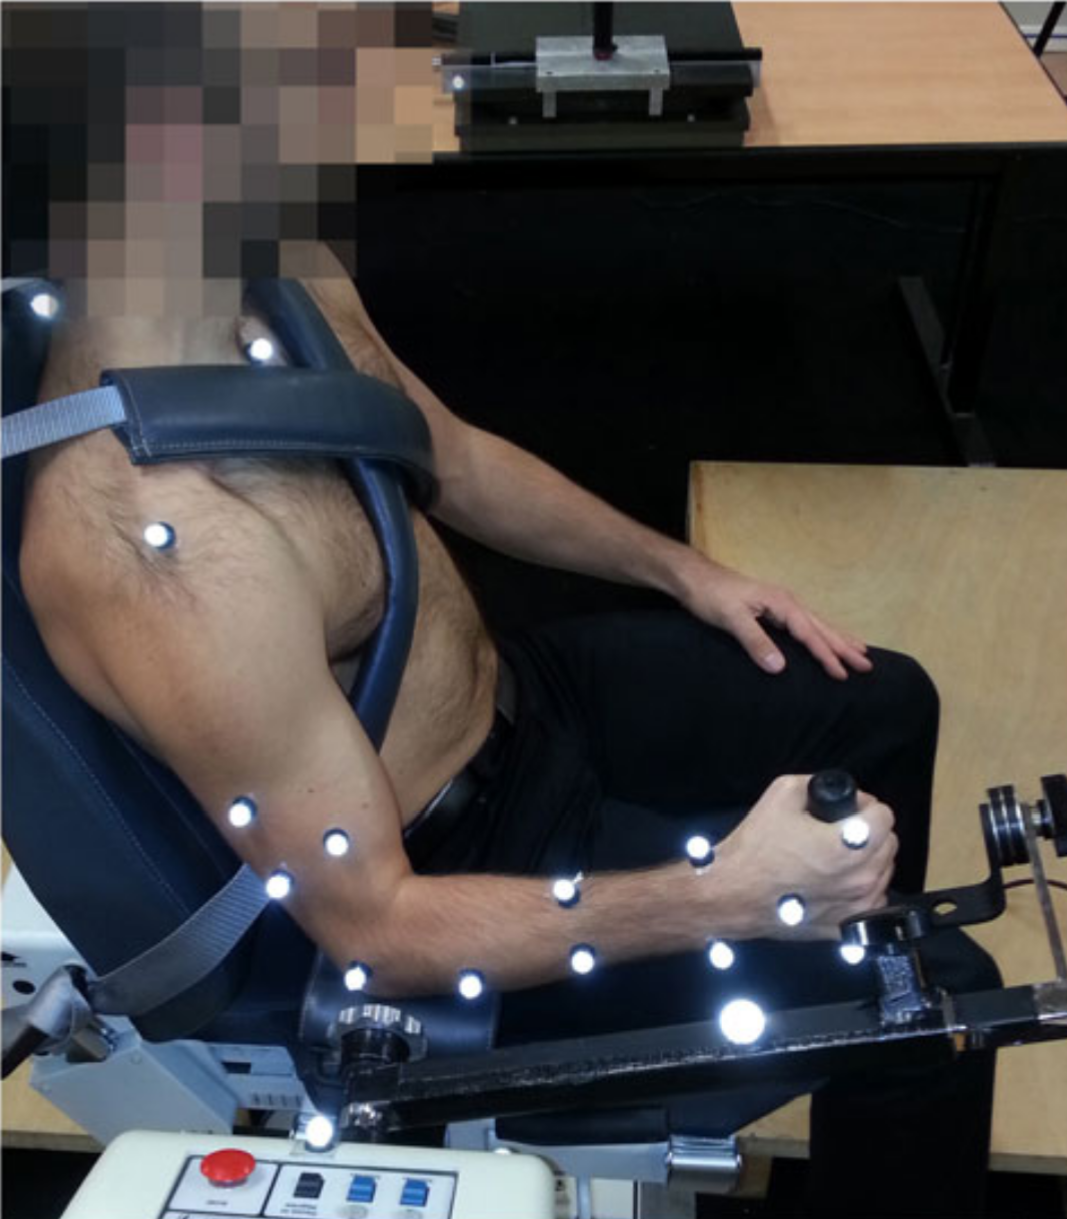
\includegraphics[trim={0 0 0 0},clip,width=0.4\linewidth]{img/chapter_1/hernandez_optoelectronic.png}
    \caption{Reflective markers placed on the upper-limb (\cite{hernandezHumanUpperlimbForce2016a}).}
    \label{fig:hernandez_opto}
\end{figure}

\paragraph*{Force directions.} The choice of directions for exerting MVICs varies depending on the posture and the desired range of force directions (a line, a plane, or the entire 3D space). 

While predicting force amplitude in a specific direction is of strong interest for characterizing individual force capabilities, this thesis focuses on understanding the underlying muscle tension interactions that generate these forces. Previous studies have explored various approaches for predicting maximal force exertion in regard to a specific direction, such as using artificial neural networks to relate upper-limb posture and anthropometric data (\cite{ladelfaArmForceField2017a}; \cite{ladelfaPredictingManualArm2016b}) or employing parametric equations to predict maximum hand force based on hand location relative to the shoulder (\cite{ladelfaEquationsPredictFemale2014a}). However, these studies do not seek to characterize how muscle tensions interact to produce these forces. As this thesis will focus this characterization, we do not expand on the predicting aspect of maximal force exertion and focus on the chosen directions within experimental procedures. 

As experimentally observed in (\cite{jannijhofMaximumIsometricArm2006a}), in which six participants were asked to exerted maximal forces at the hand in eight directions of the workspace in five different hand locations on the transverse plane, the maximum produced forces systematically depended on the hand location and the direction of exertion.

In (\cite{oshimaRoboticAnalysesOutput2000}), the authors investigated forces exerted at the hand in the transverse plane. In this 2D condition, they measured maximal voluntary isometric contractions from four subjects, with exertions performed in various directions within the horizontal plane. Each exertion lasted 1 to 2 seconds, and measurements continued until a sufficient number of directions were sampled. The subjects gripped a horizontal handle, and two postures were considered. However, the authors did not specify whether a resting period was included between measurements or how many directions were considered sufficient. 

In (\cite{sasakiHigherDimensionalSpatial2010a}), 2D force exertions in the transverse plane at the hand were also investigated, using 7 postures and a single participant. A handle was attached to a mechanical mechanism to allow for different wrist postures. In this work, 8 force directions were considered, as described in Figure \ref{fig:sasaki_foce}.
\begin{figure}[!htb]
    \captionsetup{justification=centering}
        \centering
        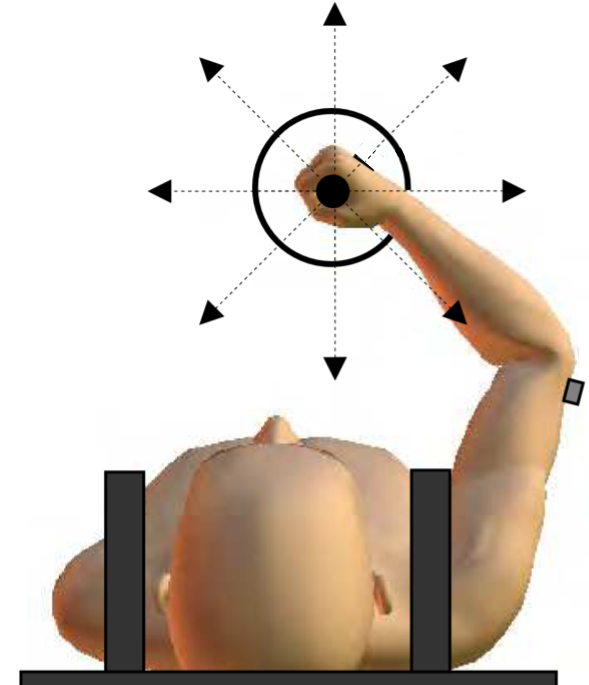
\includegraphics[trim={0 0 0 0},clip,width=0.4\linewidth]{img/chapter_1/sasaki_force.png}
    \caption{Hand force exertion directions used in (\cite{sasakiHigherDimensionalSpatial2010a}).}
    \label{fig:sasaki_foce}
\end{figure}

In contrast to the previous 2D studies, in (\cite{rezzougUpperLimbIsometricForce2021b}) the authors considered seven participants exerting maximal isometric forces in the whole 3D space, using a single posture. This posture involved slight shoulder flexion, an elbow flexed at 70°, and forearm pronation-supination at 80°. Participants exerted maximal isometric forces on a vertical handle attached to a dynamometer in 26 specified directions. These directions were defined as combinations of azimuth angles (ranging from 0° to 315° relative to the horizontal forearm axis in 45° steps) and elevation angles (-45°, 0°, and 45° relative to the horizontal plane). Two additional vertical directions, corresponding to 90° and -90° elevation, were also included. Each maximal force exertion was held for 3 seconds, with a 3-minute resting period between trials.

Similarly, (\cite{hernandezIsometricForceCapabilities2015}) employed a similar protocol, using the same 26 force directions. In their study, participants exerted maximum force for 3 seconds with verbal encouragement. Resting periods lasting 3 minutes were also included between trials.
\begin{figure}[!htb]
    \captionsetup{justification=centering}
        \centering
        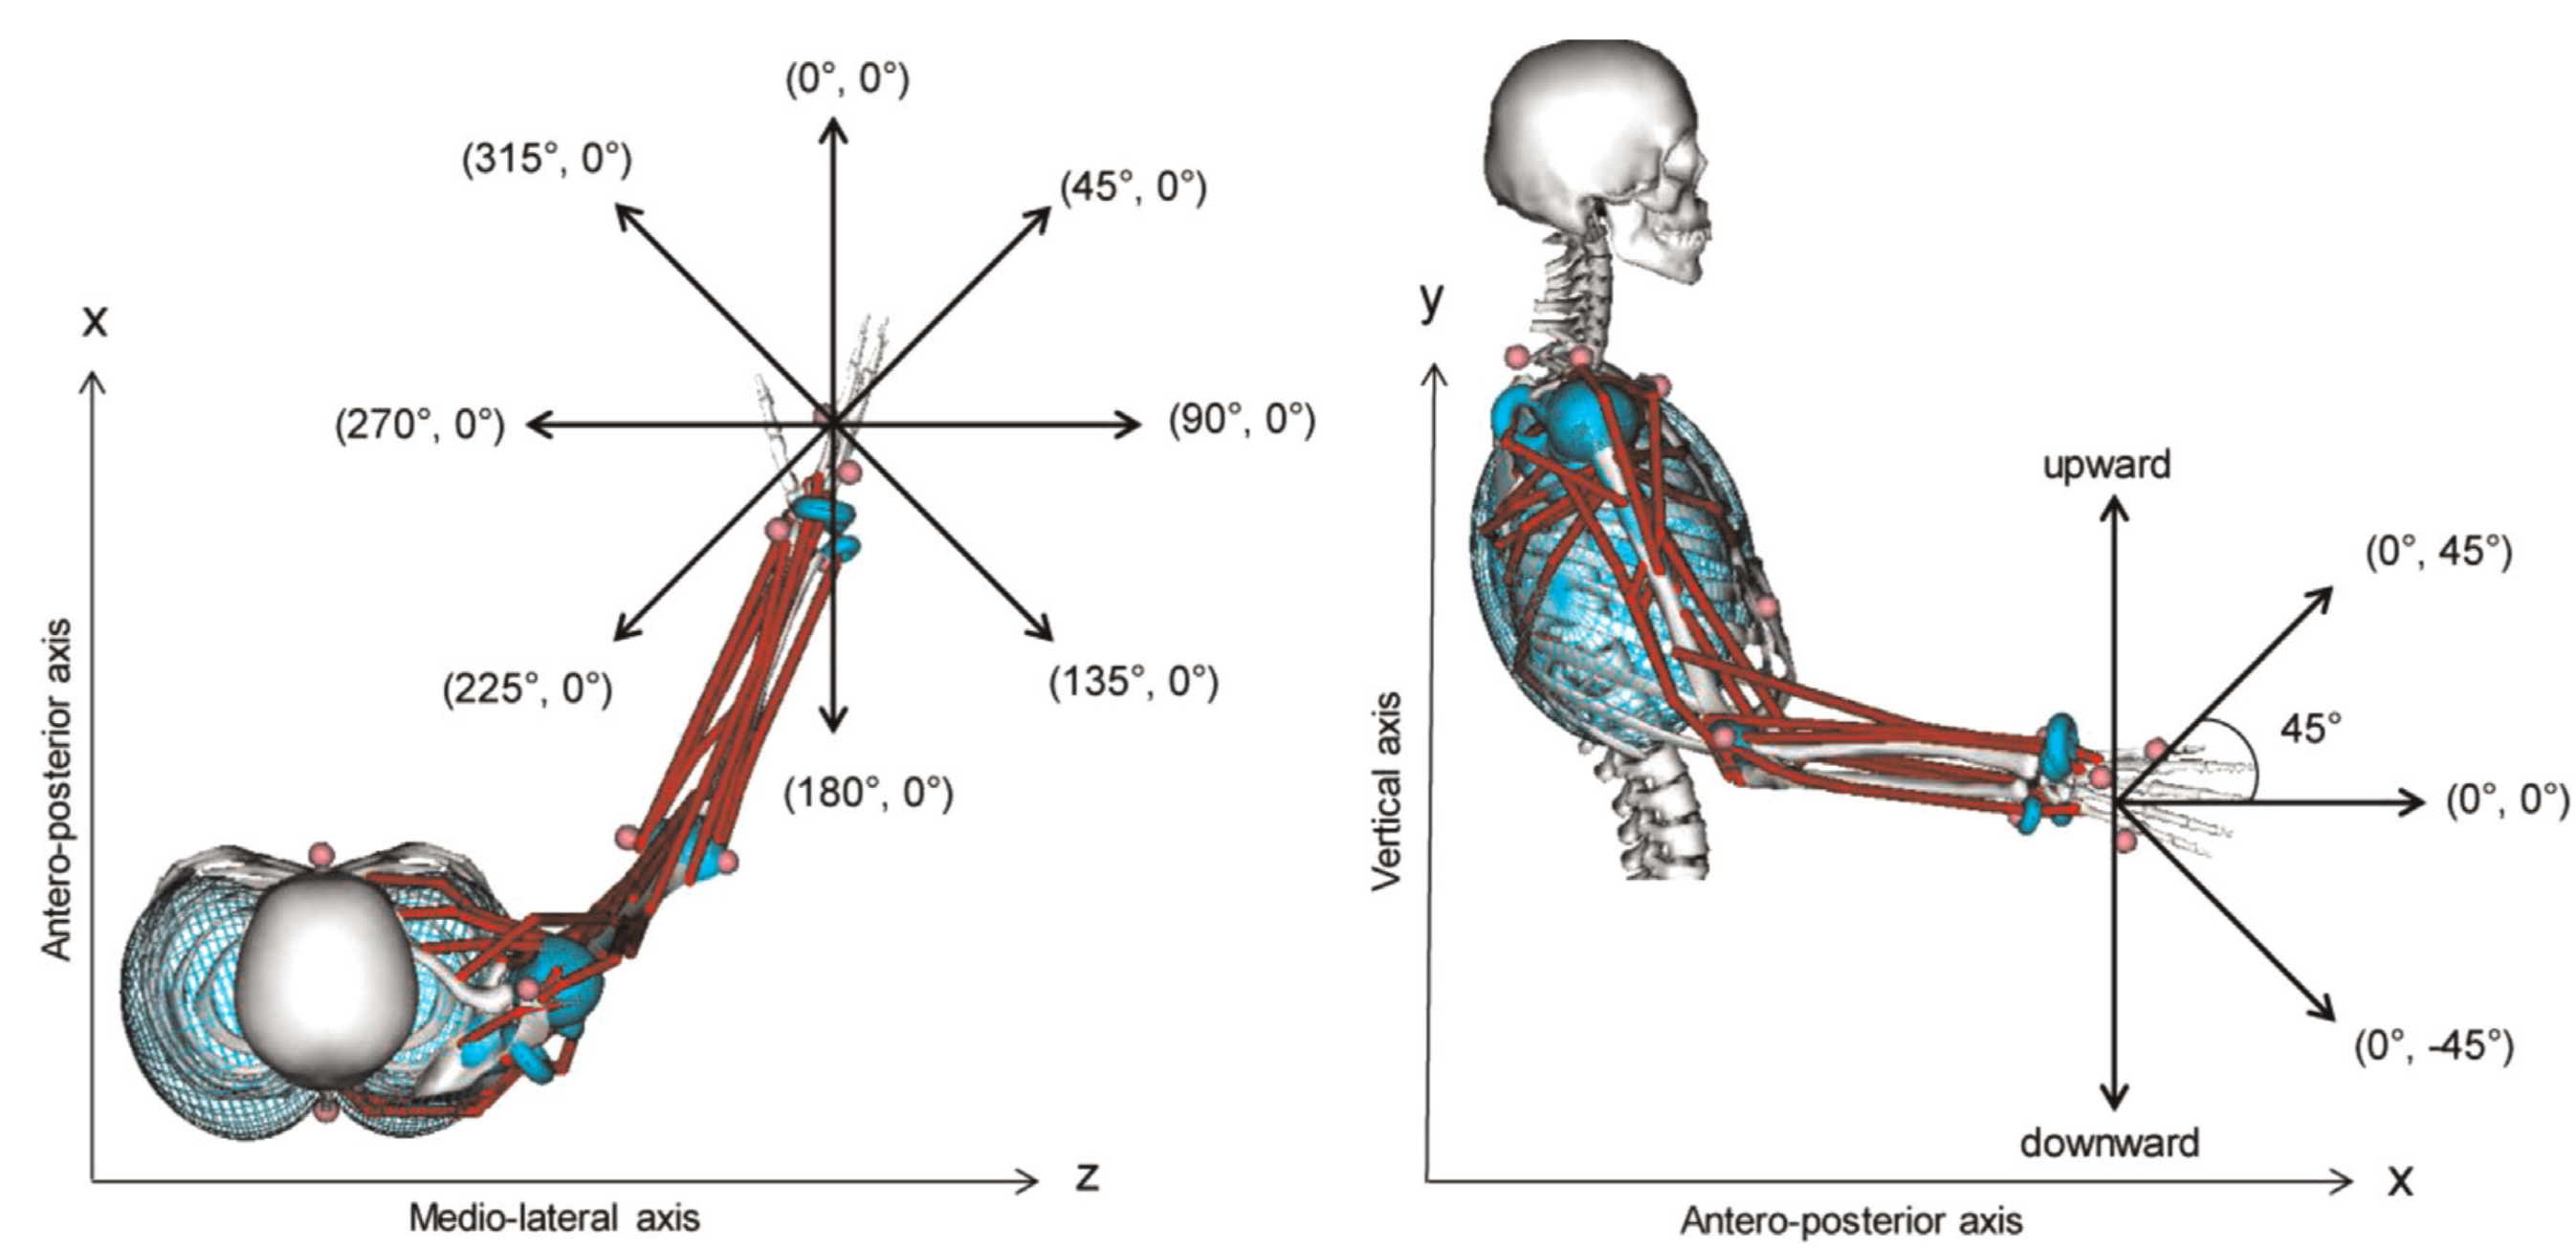
\includegraphics[trim={0 0 0 0},clip,width=1\linewidth]{img/chapter_1/axis_hernandez_rezzoug.png}
    \caption{The 26 force directions used in (\cite{rezzougUpperLimbIsometricForce2021b}) and (\cite{hernandezIsometricForceCapabilities2015}), defined by combinations of azimuth (left figure) and elevation (right figure) angles. Images from (\cite{hernandezIsometricForceCapabilities2015}).}
    \label{fig:rezzoug_hernandez_directions}
\end{figure}

As this review has shown, the inherent challenges of measuring maximal voluntary isometric contractions (MVICs) are reflected in the difficulty of estimating force feasible sets, which require multiple successive MVICs in a given posture. The required resting times between measurements result in lengthy experimental protocols, which become even longer as the number of force directions increases. These challenges may explain why the literature lacks studies with a sufficient number of MVICs measured in a single posture. Furthermore, the number of force directions chosen is often arbitrary, aiming to capture the three-dimensional nature of the Cartesian force space. Consequently, there is a need to improve experimental conditions and to gather more force data in a given posture. This would help in understanding how force capabilities vary across individuals.

This thesis addresses these challenges by making two main contributions. Chapter \ref{chapter:3} will demonstrate that in the human upper limb, the high number of muscles leads to a high probability that force feasible sets resemble ellipsoids. This holds under the sole condition that muscle tension interactions are modeled as convex. Since any 3D ellipsoid can be uniquely determined by 9 arbitrary points on its surface (5 points for a 2D ellipsoid), this result implies that measuring a force feasible set experimentally becomes less challenging. Furthermore, to address the lack of maximal force exertion data in the literature, Chapter \ref{chapter:5} will provide measurements of force feasible sets in four different postures for ten subjects.

% \subsection{\emph{In silico} force feasible set limitations towards \emph{in vivo} measurements}
\subsection{Comparison between \emph{in silico} and \emph{in vivo} force feasible sets}
\label{subsec:force_measurements_vs_ffs}
In experimental protocols where MVICs are gathered in multiple directions, the measured force feasible set is constructed as the convex hull of all measured maximal forces (\cite{oshimaRoboticAnalysesOutput2000}; \cite{rezzougUpperLimbIsometricForce2021b}; \cite{hernandezIsometricForceCapabilities2015}). However, there are examples where a set-theoretic approach is not preferred, and maximal forces are considered individually for each direction (\cite{sasakiHigherDimensionalSpatial2010a}).

Although there is a general framework for defining force feasible sets in static postures, in practice, this framework is often simplified or adapted based on biomechanical assumptions. As highlighted in (\cite{sutjiptoComparisonStrengthProfile2024a}), it is ``unclear which methods best suit modelling and representing limb strength''. We will now examine these assumptions in the context of different force feasible set representations.

In (\cite{chiacchioForcePolytopeForce1997}), the authors considered both the polytopic and ellipsoid representations of force feasible sets for a redundant general manipulator, where the number of degrees of freedom exceeds the dimension of the Cartesian space. The key difference from the general formulation presented in Section \ref{sec:muscu_model_in_silico_ffs} is that their analysis focuses solely on serial kinematic chains, which do not require the consideration of muscle and consequently tension feasible sets. For example, they define the force polytope $\mathcal{P}$ in the torque space as:
\begin{align*}
    \mathcal{P} = \im{J^T} \cap \mathcal{O}_{\tau}
\end{align*}
where $\mathcal{O}_{\tau}$ is an orthotope (hyperrectangle) whose principal axes are aligned with the canonical basis of the torque space. Furthermore, this orthotope is assumed to be centered at the origin. If this specific force polytope construction were generalized to include muscles, it would imply a one-to-one correspondence between muscles and joint torques, with each muscle acting exclusively on a single joint.

Similarly, based on the work of (\cite{yoshikawaManipulabilityRoboticMechanisms1985}), these authors define a force ellipsoid E in the torque space as:
\begin{align*}
    \mathcal{E} = \im{J^T} \cap \mathcal{E}_{\tau}
\end{align*}
where $\mathcal{E}_{\tau}$ is a $n$-dimensional axis-aligned ellipsoid in the torque space. The same interpretation as with $\mathcal{P}$ is possible, implying a one-to-one correspondence between muscles and joint torques if this construction were generalized to include muscles.
\begin{figure}[!htb]
    \captionsetup{justification=centering}
    \begin{minipage}{0.48\linewidth}
        \centering
        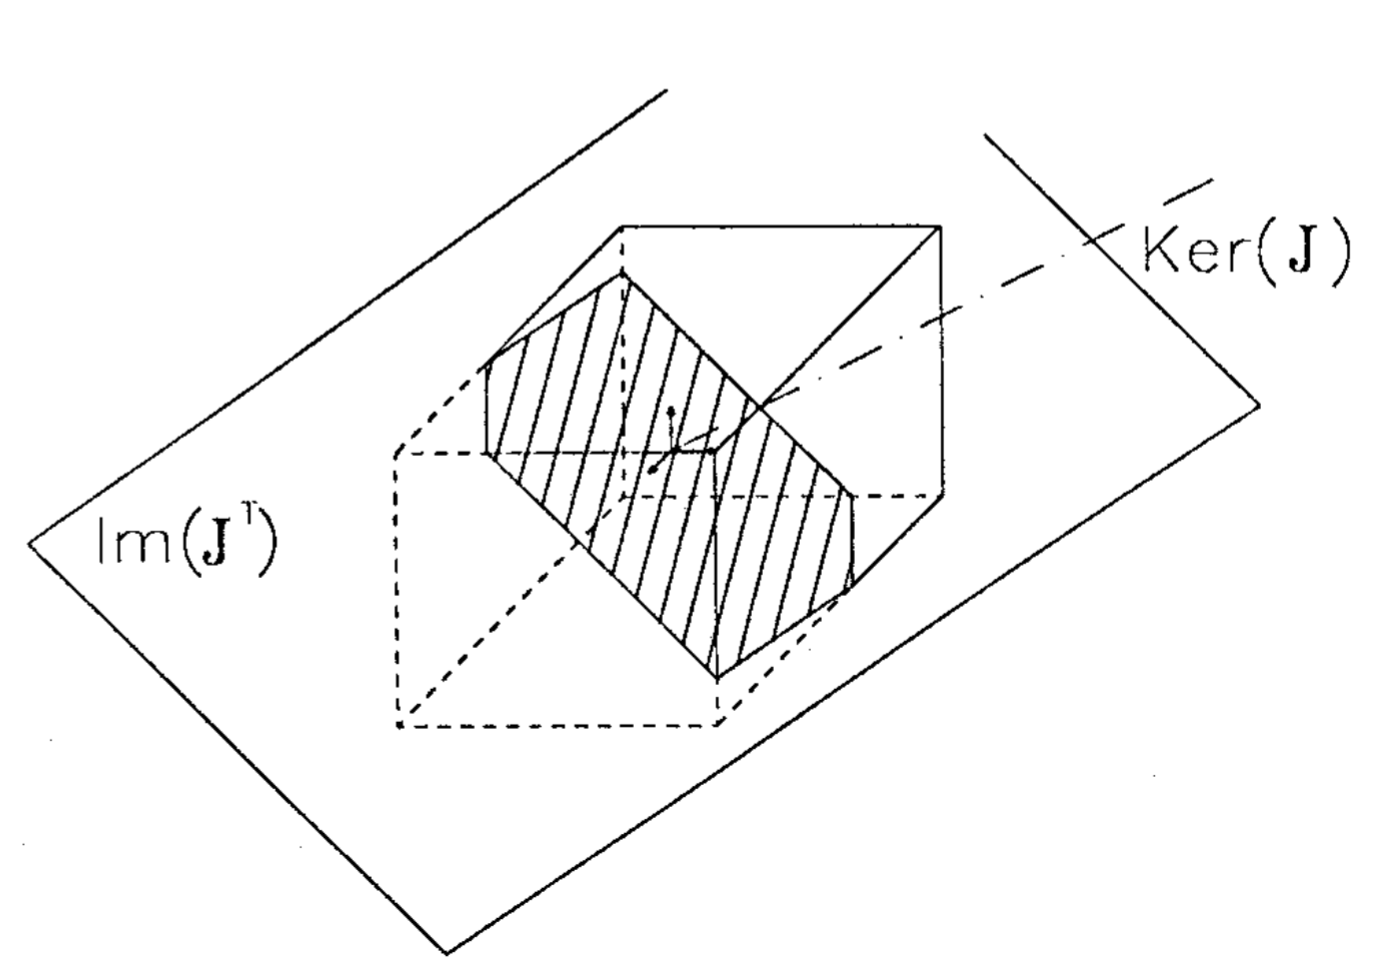
\includegraphics[trim={0 0 0 0}, clip, width=1\linewidth]{img/chapter_1/chiaccho_pol.png}
    \end{minipage}
    \hfill
    \begin{minipage}{0.48\linewidth}
        \centering
        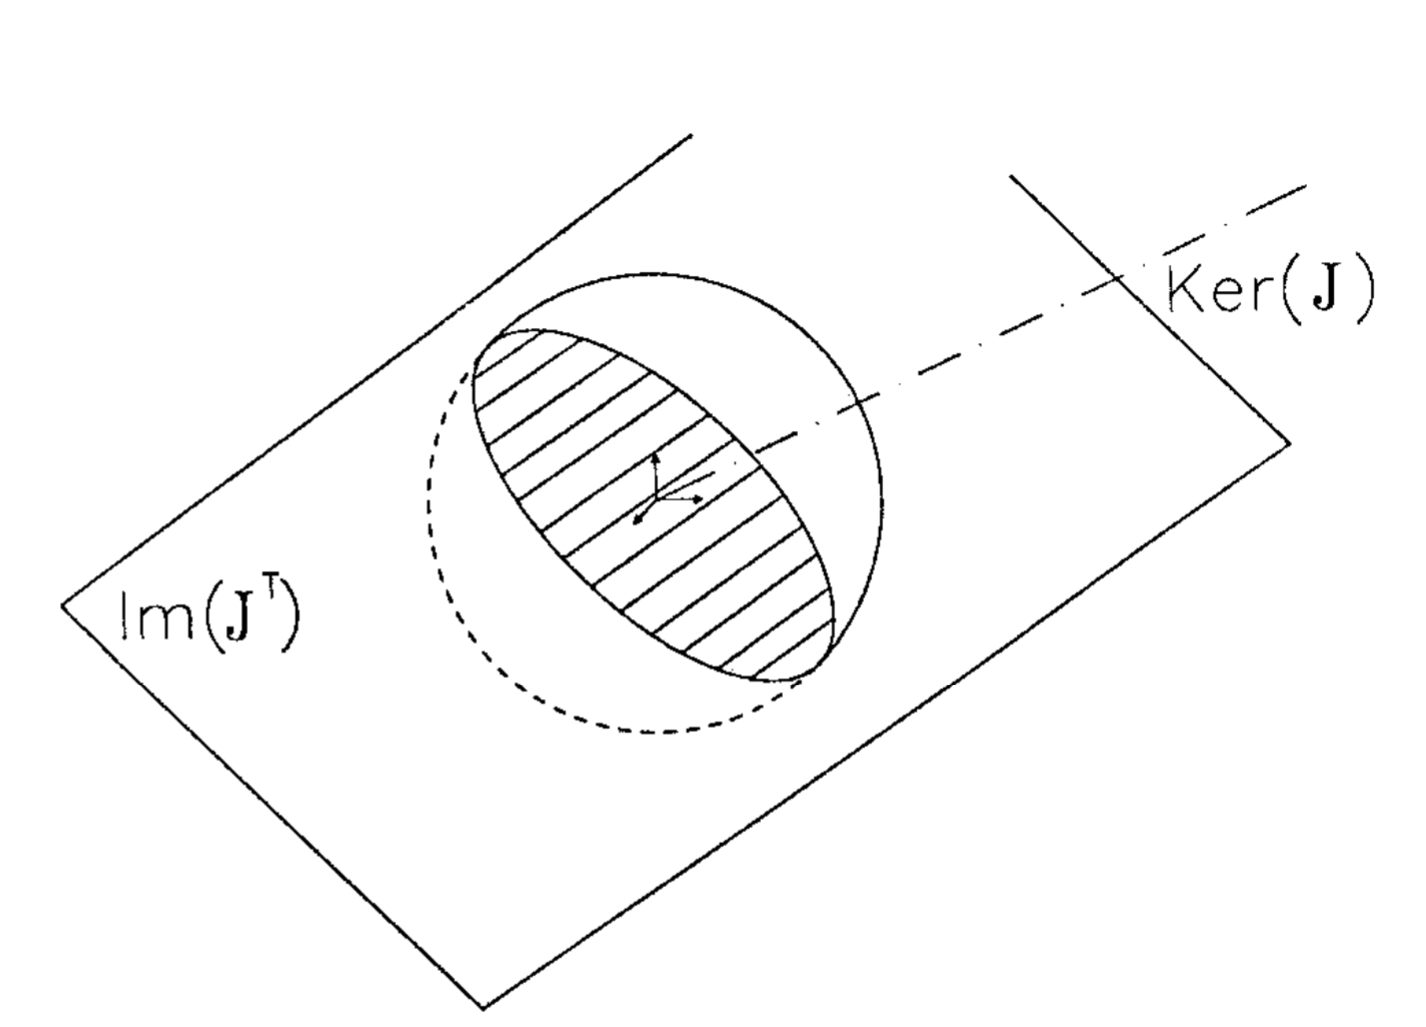
\includegraphics[trim={0 0 0 0}, clip, width=1\linewidth]{img/chapter_1/chiaccho_elli.png}
    \end{minipage}
    \caption{In dashed lines, the force polytope (left) and force ellipsoid (right) construction from (\cite{chiacchioForcePolytopeForce1997}).}
    \label{fig:chiacchio_pol_ell}
\end{figure}

The key difference between these two representations lies in the underlying notion of a norm. In the polytope case, the torque feasible set is an orthotope, obtained by a linear transformation of the unit cube $\mathcal{C} = [-1,1]^n$. This unit cube can be defined as the unit ball $\mathcal{B} = \{\mathbf{x}\in\IR^n \mid \| \mathbf{x} \|_{\infty} \leq 1 \}$ with respect to the infinity norm, where $\|\mathbf{x}\|_{\infty} = \max_i \vert x_i \vert$. Similarly, in the ellipsoid case, the torque feasible set is an ellipsoid, obtained by a linear transformation of the unit ball $\mathcal{B} = \{\mathbf{x}\in\IR^n \mid \| \mathbf{x} \|_{2} \leq 1 \}$ with respect to the Euclidean norm (also termed 2-norm), where $\|\mathbf{x}\|_2 = \sqrt{x_1^2 + \dots + x_n^2}$. Therefore, the different shapes of the force feasible sets in Chiacchio et al.'s work are determined by the choice of norm on the torque space. These norms reflect the degree of independence between the torques. The infinity norm implies complete independence, while the Euclidean norm allows for some interdependence.

Although their representations are specific to pure serial kinematic chains, introducing muscles should lead to different shapes for the torque feasible set. This is primarily because the upper limb has more muscles than degrees of freedom. Therefore, the next example, based on Chiacchio et al.'s construction, investigates the validity of assuming a simpler muscle representation in the upper limb.

(\cite{rezzougUpperLimbIsometricForce2021b}) aimed to demonstrate that the representations proposed by Chiacchio et al., when adjusted based on experimental maximal force and joint torque measurements, do not accurately capture the volume of force feasible sets in the upper limb. They constructed the force feasible set as the convex hull of maximal force measurements taken in 26 directions at the hand. The authors adjusted their \emph{in silico} geometric construction using data from two measurement sessions: one for maximal isometric force exertions at the hand in 26 directions and another for maximal isometric joint torques. Considering 7 degrees of freedom for the upper limb (3 for the shoulder, 1 for the elbow, and 2 for the wrist), they defined the \emph{scaled} force polytope $\mathcal{SP}$ as:
\begin{align*}
    \mathcal{SP} = \im{J^T} \cap \mathcal{O}_{\tau}
\end{align*}
such that $\mathcal{O}_{\tau} = \left([\tau_1^-, \tau_1^+]\times \dots \times [\tau_7^-, \tau_7^+]\right)$ is a 7-dimensional orthotope (hyperrectangle) in the torque space. For each joint $i = 1, \dots, 7$, $\tau_i^- < 0$ represents the maximal measured joint torque in the negative diretion of the joint torque's axis, and $\tau_i^+ > 0$ the maximal joint torque in the positive direction. 

They also defined the \emph{scaled} force ellipsoid $\mathcal{SE}$ as:
\begin{align*}
    \mathcal{SE} = \left(\im{J^T} \cap \mathcal{E}_{\tau}\right) + \overline{\mathbf{f}}
\end{align*}
where $\mathcal{E}_{\tau}$ is the 7 dimensional axis-aligned ellipsoid centered at $0$, with each semi-axis having length $(\vert \tau_i^-\vert + \vert \tau_i^+ \vert)/2$ for $i=1,\dots, 7$. Since there is no reason for $\mathcal{E}_{\tau}$ to be centered at 0 (because $\vert \tau_i^-\vert$ is generally not equal to $\vert \tau_i^+\vert$), the authors compute the intersection $\im{J^T}\cap \mathcal{E}_{\tau}$ and then translate it by an offset $\overline{\mathbf{f}}$. This offset is determined experimentally as the center of the ellipsoid obtained by applying singular value decomposition to the measured force exertions.

One of the key findings of this study was that both force feasible set constructions can either overestimate or underestimate the volume of the measured force feasible set. This suggests that the choice of norm for the joint torques (the max norm for the orthotope and the Euclidean norm for the ellipsoid) significantly influences the volume of the resulting force feasible set models.
\begin{figure}[!htb]
    \captionsetup{justification=centering}
        \centering
        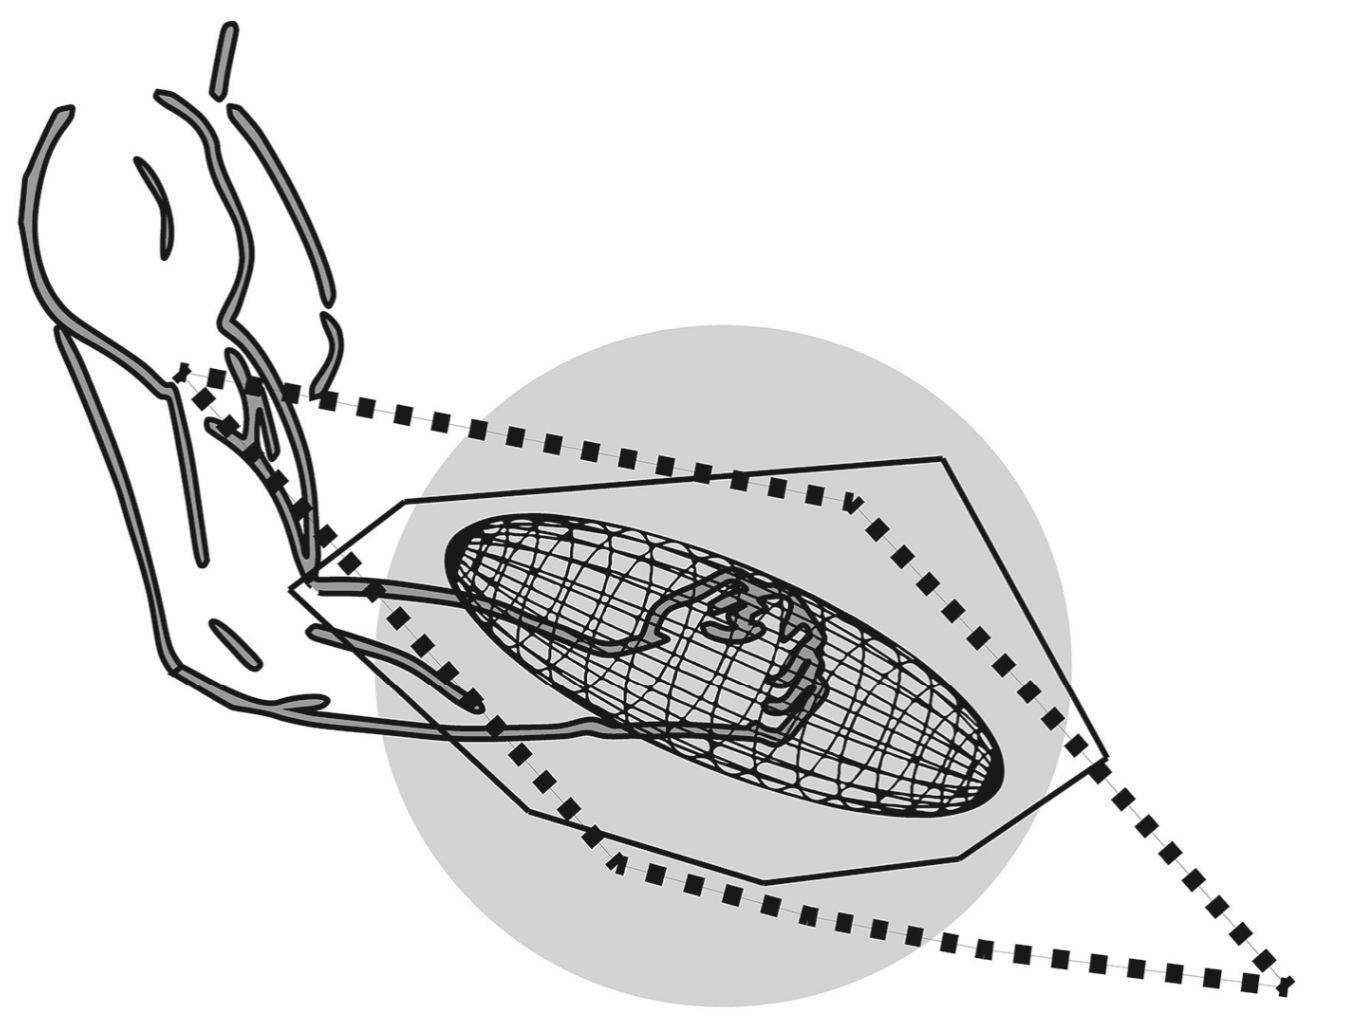
\includegraphics[trim={0 0 0 0},clip,width=0.4\linewidth]{img/chapter_1/rezzoug_2021.png}
    \caption{Representations of the simulated scaled force ellipsoid (wire-frame) and scaled force polytope (black squares) with measured force feasible set described in the sagittal plane in (\cite{rezzougUpperLimbIsometricForce2021b}).}
    \label{fig:rezzoug2021}
\end{figure}

This study also suggests the importance of considering a higher number of muscles than degrees of freedom to achieve a more physiologically accurate model of the upper limb.

To address this, in (\cite{hernandezIsometricForceCapabilities2015}) a scaled musculoskeletal model with 29 muscles and 7 degrees of freedom was used (adapted from the upper-limb model from (\cite{holzbaurModelUpperExtremity2005})) for 9 subjects. Similar to (\cite{rezzougUpperLimbIsometricForce2021b}), they used 26 force directions at the hand to gather experimental MVICs, and the convex hull of these measurements formed the measured force feasible set. For the \emph{in silico} analysis, they used a force polytope representation and incorporated muscle activations. They determined whether each muscle should be fully activated or not based on the direction of the exerted force. For a given posture and force direction $\mathbf{v}\in\IR^3$, they computed the moment arm matrix $-L^T \in \IR^{7\times 29}$. Each column of this matrix corresponds to the moment vector of a muscle. For each muscle, they orthogonally projected its moment vector onto $\im{J^T}$ and compared the angle between this projection and $J^T\mathbf{v}$. They assumed that a muscle contributes to a force direction $\mathbf{v}$ if its moment vector is aligned with $J^T\mathbf{v}$. This alignment is determined by the angle between the two vectors. If this angle is less than 90°, the corresponding muscle is fully activated (activation = 1); otherwise, it is not activated (activation = 0). They considered a large number of force directions $\mathbf{v}\in V$, with spherical coordinates $(\theta, \phi)$ where $\theta \in [0, 360$°$]$ and $\phi\in[0,180$°$]$ in 1° increments. This allowed them to characterize each muscle tension based on the considered force direction $\mathbf{v}$. Based on this muscle activation model, they defined the force polytope $\mathcal{MSFP}$ as follows:
\begin{align*}
    \mathcal{MSFP} = \left\{ \mathbf{f} \in\IR^3 \mid \mathbf{f} = (J^T)^+(-L^T\mathbf{t}(\mathbf{v}) - \mathbf{G}), \quad \mathbf{v}\in V \right\}
\end{align*}

Figure \ref{fig:hernandez2016} shows the difference between the computed force feasible set $\mathcal{MSFP}$ and the measured one for one subject in a specific posture.
\begin{figure}[!htb]
    \captionsetup{justification=centering}
        \centering
        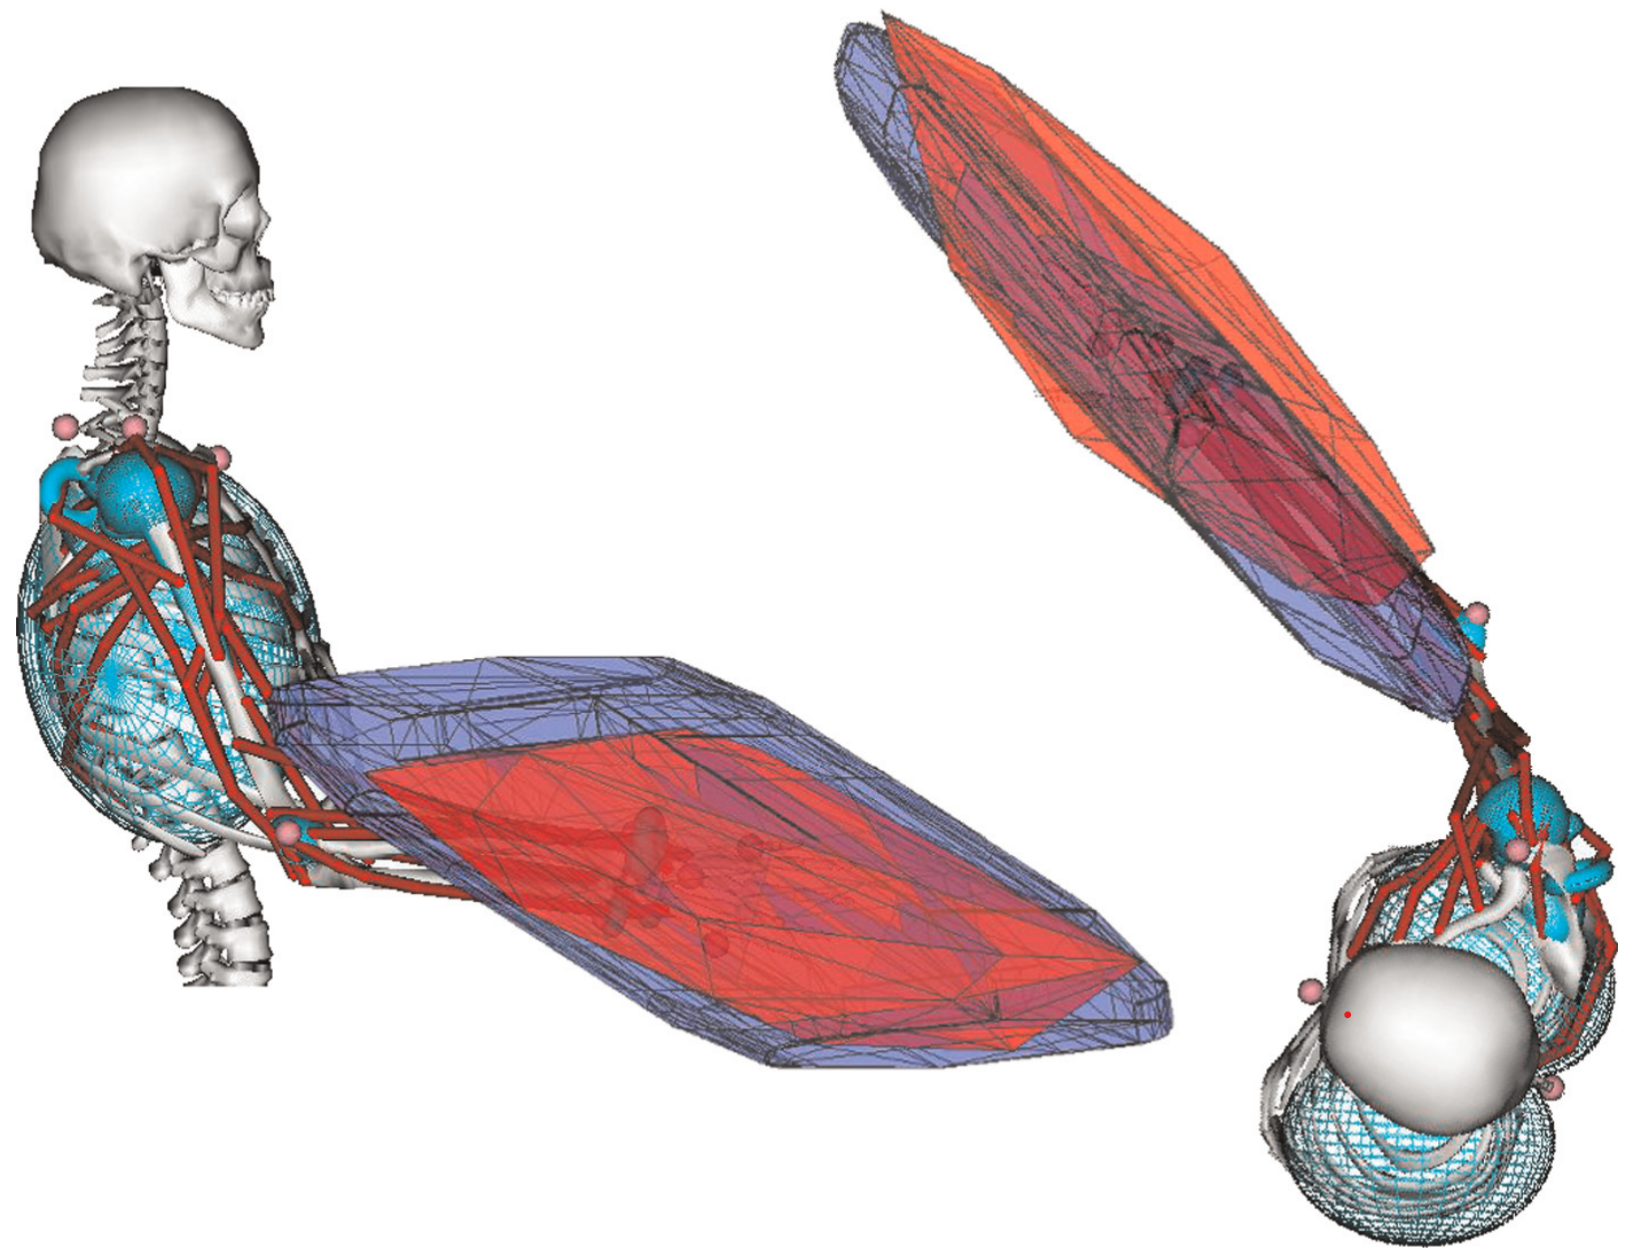
\includegraphics[trim={0 0 0 0},clip,width=0.7\linewidth]{img/chapter_1/hernandez_force.png}
    \caption{Measured (red) and computed (blue, $\mathcal{MSFP}$) force feasible sets for one subject in the sagittal plane, from (\cite{hernandezIsometricForceCapabilities2015}).}
    \label{fig:hernandez2016}
\end{figure}

Although the overall orientation of the computed force feasible set appears to be preserved, there are still significant differences in its proportions compared to the measured set. A key assumption in this experiment is that a muscle produces active tension only when it contributes to the force direction. This assumption leads to a polytopic shape of the resulting torque feasible set. The authors chose to orthogonally project (rather than intersect) the torque feasible set onto $\im{J^T}$. This choice of projection over intersection is important because it allows for a direct interpretation of the force direction with respect to the muscle joint torques. This is reflected in the authors' approach of considering specific muscle activations according to the force directions. If they had used the intersection operation instead of projection, this direct analogy between force direction and muscle activation would not be possible.

However, it is important to note that the overall orientation of the force polytopes computed by Hernandez et al. appears to be consistent with the experimental data. As shown by Hernandez et al., the angle between the principal axes of the computed and measured force feasible sets varied between 2.4° and 9.5° (in absolute value) across the subjects. This suggests that the orientation properties are largely determined by $(J^T)^+$, which is a key component of all the force feasible set formulations presented here. 

The presented studies have revealed several important properties of upper-limb force feasible sets and their representations. First, accurately modeling these sets may require considering a higher number of muscles than degrees of freedom. Second, muscle tension interactions appear to significantly influence the quality of the force feasible set, affecting its volume, elongation, and overall shape.

To further explore the shape of force feasible sets, we will now examine two studies that specifically focus on this aspect. The first study, (\cite{oshimaRoboticAnalysesOutput2000}), suggested that the set of isometric maximal forces produced at the hand in the transverse plane has a hexagonal shape. This hexagonal shape is a special case of a polytopic representation, where the forces are restricted to a 2D plane and two degrees of freedom are considered. Consequently, when the postures are not in singular joint configuration, the matrix $J^T$ is invertible, and the force feasible set becomes a linear transformation of the torque feasible set since $(J^T)^{-1}$ exists and is equal to $(J^T)^+$. However, the hexagonal shape, with its 8 edges, implies a specific constraint: only 4 muscles are present in the upper limb. The relationship between the edges of the torque feasible set and the number of muscles will be explored in more detail in Chapter \ref{chapter:2}. Although this assumption may not be physiologically accurate, it is worth noting that it could imply much simpler muscle representations for 2D force feasible sets. Similarly, (\cite{sasakiHigherDimensionalSpatial2010a}) conducted a similar experiment to (\cite{oshimaRoboticAnalysesOutput2000}), using different postures. They observed that `the feature of shape of the manipulating force polytope agrees with findings of Oshima et al. that the distribution of the hand force vector in a two-dimensional plane is a hexagonal shape', which further supports the hypothesis of a 4-muscle system.

Experimental results show that the produced hand forces can indeed be approximated by a hexagon, taking into account errors in the 8 force measurements (Figure \ref{fig:sasaki_hexagon}). This hexagonal shape was also observed in (\cite{oshimaRoboticAnalysesOutput2000}) but required a larger number of maximal force exertions to achieve it (Figure \ref{fig:oshima_force_hexagon}).
\begin{figure}[!htb]
    \captionsetup{justification=centering}
    \begin{minipage}{0.5\linewidth}
        \centering
        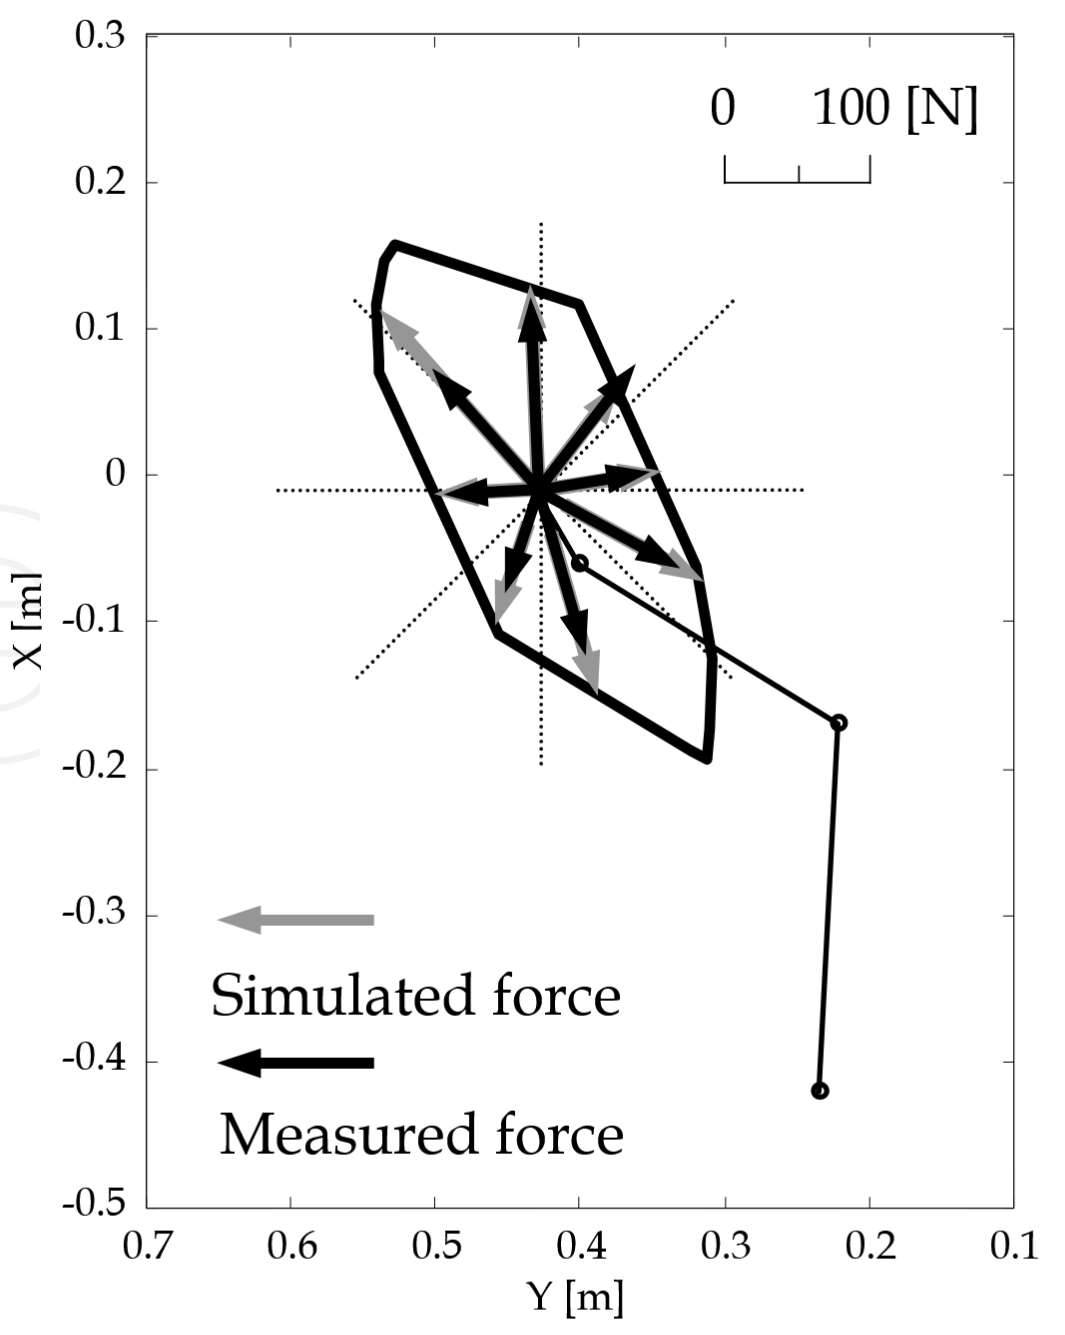
\includegraphics[trim={0 0 0 0},clip,width=0.8\linewidth]{img/chapter_1/sasaki_hexagon.png}
        \caption{Hexagon (black line) assumed in (\cite{sasakiHigherDimensionalSpatial2010a}) for 8 hand maximal force measurements (black arrows).}
        \label{fig:sasaki_hexagon}
    \end{minipage}
    \hfill
    \begin{minipage}{0.48\linewidth}
        \centering
        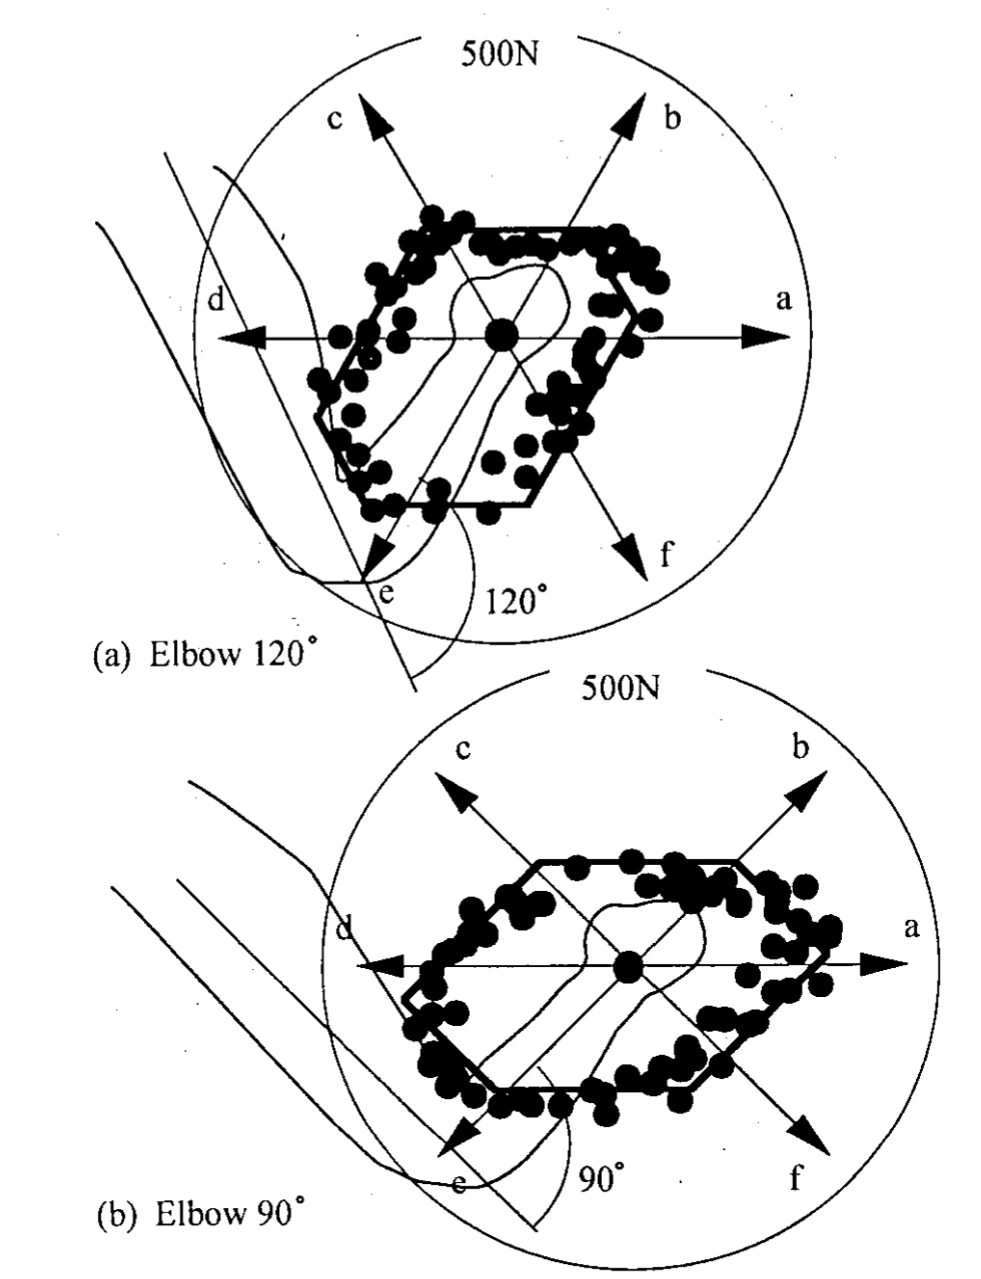
\includegraphics[trim={0 0 0 0},clip,width=0.8\linewidth]{img/chapter_1/oshima_force_output.png}
        \caption{(\cite{oshimaRoboticAnalysesOutput2000}):  maximal force measurements (black points) in two postures.}
        \label{fig:oshima_force_hexagon}
    \end{minipage}
\end{figure}

However, Oshima et al. acknowledged that an infinite number of hexagons could fit their data. Both experiments were based on prior assumptions about the number of muscles involved. It is also possible that other convex shapes with more edges, or even an ellipsoid, could have fit the experimental data equally well.


% ---------- SHOULD CORRECT ENGLISH FROM NOW
% ------------------------------------------
% ------------------------------------------
% ------------------------------------------

This subsection highlighted how inconsistencies appear between \emph{in silico} and \emph{in vivo} force feasible sets. Consequently, it is relevant to consider how accurately force feasible sets can be modeled to reflect an individual's muscles, especially given the uncertainty regarding which \emph{in silico} modeling choices best reflect \emph{in vivo} measurements \cite{sutjiptoComparisonStrengthProfile2024a}.

% This subsection highlighted how inconsistencies appear between \emph{in silico} and \emph{in vivo} force feasible sets. As such, it is relevant to consider to what extent force feasible sets can be modeled to reflect the muscles of an individual, as it is unclear which modeling choice of \emph{in silico} force feasible set may best reflect \emph{in vivo} experimental measurements (\cite{sutjiptoComparisonStrengthProfile2024a}). 

% The next subsection focuses on this challenge, and how this observed difficulty can be quantified in order to better direct the modeling of force feasible sets specifically to an individual.

% \subsection{Measuring the feasibility of musculoskeletal muscle personalization}
% \label{subsec:sensitivity_approaches}

% % \subsubsection*{La Delfa, potvin} \cite{ladelfaArmForceField2017}, \cite{ladelfaEquationsPredictFemale2014}, \cite{ladelfaPredictingManualArm2016a}


% In musculoskeletal modeling, \emph{muscle personalization} refers to the process of tailoring a generic muscle model to reflect the specific biomechanical characteristics of an individual. This involves adjusting the parameters defining the musculoskeletal model and match the individual's unique anatomy and physiology (\cite{fernandezNarrativeReviewPersonalized2023}). The newly constructed model, termed a \emph{personalized} model or a \emph{subject-specific} musculoskeletal model, is validated by comparison against experimental data, such as its capabilities to reproduce a specific movement or net joint force and moments.

% Requiring a personalized model depends on the research question, as recalled in (\cite{saxbyMachineLearningMethods2020}), where the authors argue that the use of a more \emph{generic} model is of interest when the objective is not particularly sensitive to model personalization. For instance, the study of change of muscle function after a surgical relocation of muscle attachment points does not require a personalization process (\cite{akhundovSubjectspecificMusculoskeletalModelling2022}). In the contrary, subject-specific models should be favored on a case-by-case basis, as for instance when a generic model can not properly represent \emph{in vivo} lower limb net joint moments produced by muscles in a simulated sprint and cut task (\cite{akhundovSubjectspecificMusculoskeletalModelling2022}).

% \emph{In silico} force feasible sets contain, through their set-theoretic nature, information of a posture, muscle geometry and force-generating characteristics, but also how muscles are dependent of each other activations. All of these parameters are included in their mathematical definition. As it is possible to scale a generic model to fit an individual, it can be assumed that a given upper-limb posture is known, and also the bone geometry of an individual. As such, quantifying how muscle parameters (maximal isometric force, optimal fiber length, tendon slack length, geometrical path, etc.) influences force feasible sets is a necessary step to evaluate to what extent a personalization process might be feasible. Such influence can be quantified through a \emph{sensitivity analysis}

% Evaluating the \emph{sensitivity} of a function $f\,\colon X \to Y$ consists on measuring how the \emph{topology} of $X$ affects the topology of $Y$ under $f$. The topology of a mathematical structure refers to the general notions of continuity, limits, connectedness, shape, smoothness, etc. Small changes in $X$, like tweaking a parameter, might lead to significant shifts in the topology of $Y$, indicating high sensitivity. This means the output is heavily influenced by that particular parameter. Conversely, if large changes in $X$ barely affect $Y$'s topology, the output is insensitive to those inputs. Sensitivity analysis thus comprises of methods to obtain quantitative insights on a given mapping, in order to ``draw out the maximum capabilities of mathematical modeling'' (\cite{rabitzGeneralFoundationsHighdimensional1999}). 

% % While it is natural to consider that $f$ shapes $Y$ according to $X$, a more rich (mathematically speaking\footnote{This is also referred as the \emph{fiber} theory, or the study of pre-images.}) approach consists of seeing how the variability of $X$ is according to the variability of $Y$. In other word, this approach studies the variability of $X$ as $X = f^{-1}(Y)$ where $f^{-1}$ is the pre-image mapping, which corresponds to the usual inverse of $f$ if $f$ is bijective. The first approach is termed a \emph{local} sensitivity analysis, while the second is a \emph{global} analysis (\cite{borgonovoSensitivityAnalysisReview2016}).

% There are two types of sensitivity analyses, termed \emph{local} and \emph{global} methods (\cite{borgonovoSensitivityAnalysisReview2016}). Local methods perform an analysis in a relatively small (sometimes infinitely small) neighborhood around a chosen element of the domain $X$. This includes for instance to compute the partial differentials of a function $f$, if it is differentiable, and study the properties of its Jacobian matrix (first order differentials) and Hessian matrix (second order differentials). Other methods would involve finite differences, if $f$ is not necessarily differentiable, and \emph{screening} methods (\cite{paleariSensitivityAnalysisUsing2021}) which are more adequate when evaluating $f$ is time-consuming and/or ressource-heavy. Essentially, screening methods evaluate $f$ on a limited number of other elements around a chosen element of $X$. In our context, this would require for instance to consider a fixed parameterization of a musculoskeletal model, and create small perturbations around it to gauge how a perturbated parameter would influence the produced force feasible sets.

% On the other hand, global (or probabilistic) sensitivity methods assign a probabilitic model to describe the variability of the domain $X$ in regard to values of $Y$. These are particularly adequate methods for a general understanding of $X$ under $f$, notably it can tell us if $X$ is strongly irregular with a lot of local minima or if it a surface which consists of wide local minima largely spaced in between them. 

% With these considerations, common sensitivity analyses may not be adapted, as they usually consider a vector-to-vector and not a set-to-set relationship. As such, we focuses on the challenges induced by the set-theoretic nature of force feasible sets for sensitivity analyses. 

% Therefore, this section serves as introducing methodologies to evaluate how muscle parameters influence force feasible sets, in order to determined to what extent a musculoskeletal model personalization process may induce difficulties using force feasible sets. In this regard, Chapter \ref{chapter:4} will thus provide an adapted sensitivity analysis, based on a personalization process, which will lead to better characterization of these challenges.

% % First hints have been experimentally shown that these sets proportions vary according to an individual. For instance in (\cite{hernandezIsometricForceCapabilities2015}), the authors measured maximal isometric forces in various directions for nine participants, and the resulting measured force feasible sets were shown to be different in shape, and global size, compared to \emph{in silico} force feasible sets. 

% % When referring to a personalized model in this chapter, we shall strictly consider the personalization of a \emph{musculoskeletal model} and its parameters describing muscle force models and produced torques. For instance, the following study implies, in a sense, the personalization of a model which is a curve: \cite{aldiniRealtimeEstimationStrength2021} propose a 4 dimensional curve to modelize the \emph{strength capacity} of the hand. Their goal was to create a parametric equation (with respect to the pose of the upper limb) to model the strength capacity at the hand of an individual in a context of physical Human-Robot collaboration of an operator's hand and a robot end-effector. They assumed the feasible tension set to by an orthotope. The strength fitting was made offline on 910 hand positions. The direction of the force for each pose is fixed for each pose, and defined to be along the direction from the hand to the thorax centre. DOFs at the wrist were ignored. The resulting curve, for each of the 6 participants, seemed to predict the variations in amplitude of the measured forces, and this approach presents an average RMSE for all 6 participants of $37.67\pm 8.02$ N between the created curves and experimental measurements in 13 different postures. As the authors mentionned, this could be due to loss of accuracy in the positions. This method is thus a parametric personalization of a musculoskeletal model in order to study exerted maximal forces in specific directions depending on the individual posture.

% % While relevant in practice, this type of personalization do not allows to consider other force directions at the same time.



% % In (\cite{delpInteractiveGraphicsbasedModel1990a}), it was studied how, in the lower limb, the muscle path (represented as a series of line segments) as well as the musculotendon parameters (maximal isometric force, optimal fiber length and tendon slack length) influence the generation of each muscle joint force and moment. For this sensitivity analysis, the authors considered that a muscle to span a 1-degree of freedom revolute joint, and they perturbated the tendon slack length, the optimal fiber length, as well as the joint angle at which the maximal isometric muscle force is produced for a given muscle. They found that depending on the ratio tendon slack length/muscle moment arm, the ge TO REDO

% In (\cite{carmichaelUpperLimbStrength2015}), the authors studied \emph{in silico} how muscle parameters such as the maximum isometric force, optimal fiber length and tendon slack length influence the exertion of a maximal force at the hand in 14 different directions, for 46 hand locations while keeping the trunk fixed. They considered Holzbaur's upper limb model (\cite{holzbaurModelUpperExtremity2005}) and locked the wrist and finger joints, leaving 3 degrees-of-freedom in the shoulder and 1 in the elbow. They effected a local sensitivity analysis so that they perturbated one muscle parameter by perturbating it by $\pm 1\%$ from its original parameter's value to consider an approximation of the partial derivative function returning the maximal exerted force magnitude. For each direction and posture, they evaluated the sensitivity index $\varepsilon_{p_M}$ of the muscle parameter $p_M$ of muscle $M$ as:
% \begin{align*}
%     \varepsilon_{p_M} = \left| \frac{(S_{p_M}^+ - S_{p_M}^-) / S_{p_M}^0}{(p_M^+ - p_M^-)/p_M^0} \right|
% \end{align*}
% where $S_{p_M}^0$ is the maximal exerted force magnitude computed with no variation of the initial parameter value $p_M^0$, $S_{p_M}^+$ is the magnitude computed with a $1\%$ variation of the initial parameter value ($p_M^+$) and $S_{p_M}^-$ is the magnitude computed with a $-1\%$ variation of the initial parameter value ($p_M^-$). 

% The authors concluded this experiment by comparing the sensitivity of parameter types for all muscles, so that the tendon slack length and the optimal fiber length seem to be the most sensitive, then followed by the maximal isometric force of muscles and the pennation angle. They also conducted the same experiment with perturbations of $\pm 5\%$, which led to the same conclusion. This study goes much further and focus on how much more sensitive are the parameters in pathological cases, but we focus on the methodology more than the conclusions. 

% A similar method based on slightly perturbating muscle parameters can be found in (\cite{delpInteractiveGraphicsbasedModel1990a}) to characterize how muscle geometric and force-generating parameters affect maximal produced joint torques. 

% Also, (\cite{flores-hernandezScapulothoracicRhythmAffects2019}) studied the sensitivity of the shoulder motion for glenohumeral joint forces to show that it does have an impact. 

% Lindbeck et al., 2023 \cite{lindbeckPredictionsThumbHand2023}

% These experiments perturbated one parameter at a time. When considering exert.

% Global sensitivity analyses seem to be more rare in the literature, as they necessarily involve more computational ressources. Nevertheless, a study from 2006 by Langenderfer et al. cite{langenderferProbabilisticModelGlenohumeral2006} considered multivariate Gamma distributions to probabilistically simulate the effects of variability in PCSAs, moment arms and the muscle length-tension relationships for muscle accross the shoulder. They considered tendons to be rigid. In other words, their method consist on modeling the intra-variability of characteristics of multiple shoulder muscles in cadaveric specimens by Gamma distributions, and correlate them with the intra-variability of experimentally measured force and joint torques over the glenohumeral external rotation of 120 healthy subjects, in a specific posture. The posture considered the elbow to be flexed at $90$°. Subjects  were asked to perform voluntary maximal isometric effort around the shoulder external rotation axis.

% They evaluated the sensitivity of these parameters towards the developped muscle forces and joint torque over the glenohumeral external rotation. Tendons were modeled as rigid. Experimental glenohumeral strength force and moment were gathered for 120 healthy individuals (60 males, 60 females) in a upper limb posture with 90° elbow angle, performing maximal effort around the shoulder external rotation axis. Also, the authors gathered characteristics of 3 shoulder muscles (supraspinatus, infraspinatus and teres minor). They gathered each muscle moment arms in the reference posture for 10 glenohumeral cadaver specimens. They also gathered the optimal fiber length, the physiological cross-sectional area and tendon slack length of each muscles in order to form a force-length relationship.

% perturbations of muscle parameters (PCSA, moment and muscle length tension relationship), look at produced muscle forces and joint torque.

% % \subsection{Personalization of muscle parameters and measurements}
% % \label{subsec:sensitivity_ffs}

% % Measurements:
% % Strength profile: \cite{sutjiptoComparisonStrengthProfile2024}
% % In the horizontal plane: \cite{jannijhofMaximumIsometricArm2006}

% % \subsubsection*{Personalization examples with exerted forces}

% % In 2000, Oshima et al. \cite{oshimaRoboticAnalysesOutput2000} considered the force feasible set (as a polytope) of a planar serial kinematic chain with 2 revolute joints to represent the upper limb shoulder and the elbow, as well as 6 muscles crossing either one joint or two. The authors wanted to identified each muscle exerted force from the produce force polytope shape. However, the fact only planar forces and 2 joints are considered means that the force polytope has the particular shape of a \emph{zonotope}. Indeed, they considered postures where the jacobian transpose matrix is invertible, so that the force feasible set is a linear transformation of the torque feasible set, represented in their case a zonotope (projection of the muscle feasible tensions hyperrectangle). Due to this specific case, they succeeded, in silico and in vivo on a single participant, through geometric reasonning on the symmetries of the edges on the zonotope surface, which are directly related to th muscle (more details will be provided in chapter \ref{chapter:2}). Also, the authors claimed that the force feasible sets produced by the individual has a zonotopic shape, where the given representations of measured forces in this article could also allow us to consider an ellipsoid representation of these measures. They acknowledge this arbitrary choice of an hexagone (a type of 2D zonotope) but stating that there could have been an infinite amount of hexagons to fit the data.
% % \begin{figure}[!htb]
% %     \captionsetup{justification=centering}
% %         \centering
% %         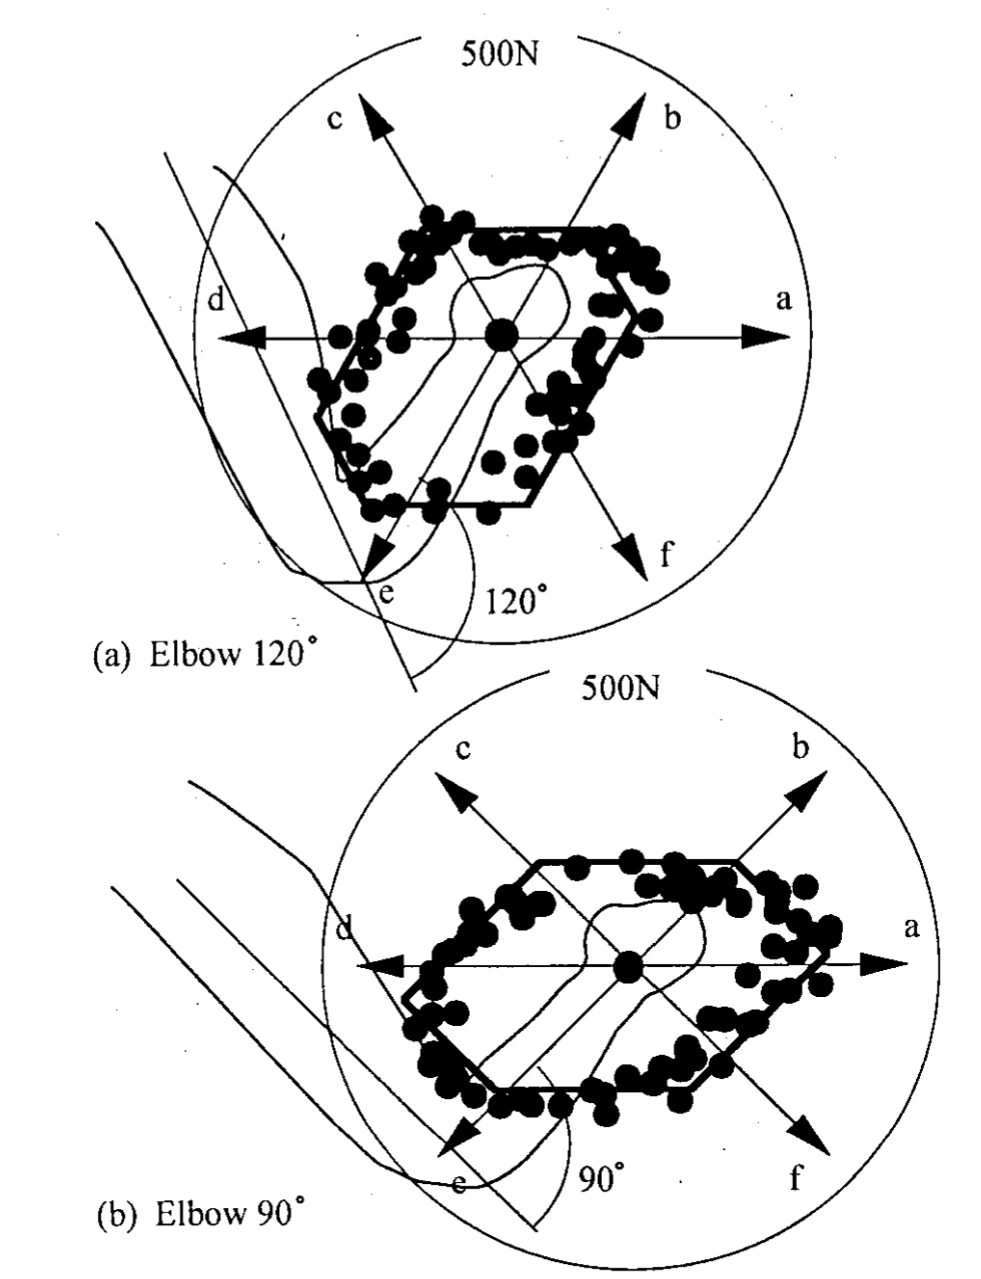
\includegraphics[trim={0 0 0 0},clip,width=0.4\linewidth]{img/chapter_1/oshima_force_output.png}
% %     \caption{Oshima et al. \cite{oshimaRoboticAnalysesOutput2000} maximal force measurements (black points) in two postures.}
% %     \label{fig:oshima_force_output}
% % \end{figure}


\subsection{Conclusion}
This subsection focused on the process of measuring maximal isometric forces at the hand in a specific posture, from the challenges of obtaining accurate maximal voluntary isometric contractions (MVICs) to the construction of \emph{measured} force feasible sets. 

The challenges associated with measuring MVICs may explain the scarcity of data on MVICs measured in different directions for a single posture. In this regard, Chapter \ref{chapter:5} details an experimental protocol for collecting MVICs in 26 different directions for 4 distinct postures in 10 subjects. 

Furthermore, there is no standardized procedure for determining the number and directions of measured forces required to adequately represent a force feasible set. Therefore, Chapter \ref{chapter:2} draws theoretical conclusions about the natural shape of a force feasible set when a large number of muscles are considered. This chapter will demonstrate that an ellipsoidal shape is sufficient to represent force feasible sets. From an experimental perspective, this reduces the number of maximal forces that need to be measured, as a 3D ellipsoid can be described by only 9 points on its surface, and a 2D ellipse by only 5. 

Finally, although there is no consensus on which force feasible set description best reflects the characteristics of maximal isometric forces, this thesis proposes a simpler theoretical representation (Chapter \ref{chapter:3}). This representation is then adapted and compared with experimental data (Chapter \ref{chapter:5}) to evaluate its relevance. Since the extent to which force feasible sets encapsulate information about muscle geometry and muscle tensions remains unclear, the next section investigates how these sets are influenced by muscle architecture and force-generating properties. 

\section{General conclusion}
This chapter encompassed a review of the literature concerned with the required biomechanical tools for a complete study of maximal isometric forces in a set-theoretic framework. First, we focused on how to model them \emph{in silico}, via force feasible sets, and showed how computational difficulties arise, necessitating the development of better computational algorithms. Second, we examined how experimental measurement of maximal isometric forces is not necessarily coherent with \emph{in silico} force feasible set models, necessitating improved modeling of force feasible sets and more judicious selection of measurement directions to mitigate experimental challenges. Finally, the chapter explored sensitivity techniques used in biomechanics, as these methods could give insights on how muscle tensions and their interactions are reflected in the set-theoretic approach of force feasible sets. The following paragraphs summarize for each section the difficulties encountered in the literature and how this thesis addresses them.

In Section \ref{sec:muscu_model_in_silico_ffs}, the dynamics of the human upper-limb were represented \emph{in silico} using a serial kinematic chain. This allowed for the description of forces applied to the upper-limb, and the \emph{force feasible set} formulation was given in a very general case as well as in isometric conditions with a fixed upper-limb posture. The construction of the force feasible set is inherently geometric: it involves the \emph{projection} of a higher-dimensional set, termed the \emph{muscle tension feasible set}, onto the torque space, which is then \emph{intersected} by a vector subspace of dimension 3. Different models, based on geometric assumptions about the muscle tension feasible set, are used to describe the force feasible set: if each muscle acts independently of other muscles, the resulting force feasible set is a 3D \emph{force polytope}. When muscle tensions are interdependent, the resulting shape is more rounded, as with \emph{force ellipsoids} (assuming an ellipsoidal tension feasible set). These representations are used in different contexts, depending on whether muscle independence is assumed (polytope) or inter-muscle dependencies are considered (typically modeled using ellipsoids). A force polytope representation is challenging to visualize, as it involves combinatorial processes to express its surface, whereas force ellipsoids are much simpler. This combinatorial increase in time complexity necessitated strategies for reducing computation time, which are explored in Chapter \ref{chapter:2}. This chapter presents a new vertex enumeration technique to describe the torque feasible set surface.

Section \ref{sec:modeling_muscle_tensions} delved into the experimental process involved in collecting maximal isometric forces, from the standardized protocol of maximal voluntary isometric contractions (MVICs), to the creation of force feasible sets from these measurements within a fixed posture. Inconsistencies in the proportions and shapes were observed between \emph{in silico} force feasible sets and experimental measurements. Since these characteristics depend on how the upper-limb is modeled \emph{in silico} (\emph{e.g.}, number of muscles, level of detail in muscle geometrical paths), Chapter \ref{chapter:3} of this thesis offers a new geometrico-probabilistic perspective on how these \emph{in silico} force feasible set characteristics behave as the theoretic complexity of a musculoskeletal model increases. As such, a unified representation of force feasible sets as ellipsoids will be computable under specific theoretical assumptions (namely, a \emph{high} number of muscles). Furthermore, Chapter \ref{chapter:4} will assess whether the biomechanically validated musculoskeletal model of the upper-limb from (\cite{holzbaurModelUpperExtremity2005}) has sufficient muscle detail to apply these assumptions in the context of muscle personalization. This section also highlighted a lack of experimental data concerning multiple maximal isometric force exertions in a fixed posture; Chapter \ref{chapter:5} addresses this by providing new experimental measurements of maximal isometric force exertions in 4 different postures for 10 participants.

% Section \ref{sec:feasibility_personalization} focused on the challenges of retrieving muscle parameters from a collection of maximal isometric forces, given the set-theoretic nature of this data. Sensitivity analysis methods used in biomechanical contexts were compared to determine the most relevant approach for considering the geometric construction of force feasible sets. Based on this comparison, Chapter \ref{chapter:4} introduces a new adapted sensitivity analysis methodology, which provides insights into the challenges of musculoskeletal model muscle personalization from force feasible sets, and demonstrates that muscle geometry parameters are not the most influential factors determining the difficulties occuring in a personalization process.

